% =====================================================================
%  YAM 415 Game Programming - Game Concept & Design Document
%  Hold the Door - Aggro Games
%  Istanbul Sabahattin Zaim University
% =====================================================================
\documentclass[10pt,a4paper]{article}

% ---------------------------------------------------------------------
%  Cover details:
% ---------------------------------------------------------------------
\newcommand{\GroupName}{Aggro Games}
\newcommand{\GroupCode}{G01}
\newcommand{\GameName}{Hold the Door}
\newcommand{\DocVersion}{v1.0}
\newcommand{\DocDate}{27.10.2026}
\newcommand{\PreparedBy}{Emir KAYA, Ömer Faruk YÜCE, Metehan GERGİN}
\newcommand{\GroupLogo}{figures/aggro_clean_td_logo.png}

% ---------------------------------------------------------------------
%  Guidance: \showguidancetrue shows the grey guidance boxes, the grey hints
%  in the tables, the examples in Appendices B-D and part 1 (Template
%  Introduction). Use \showguidancefalse for the PDF you submit; the
%  section numbers stay the same.
% ---------------------------------------------------------------------
\newif\ifshowguidance
\showguidancetrue

% =====================================================================
%  Layout of the game document template (fonts, headings, tables, cover). You do not need to edit this file.
% =====================================================================
\usepackage{iftex}
\ifPDFTeX
  \usepackage[T1]{fontenc}
  \usepackage{tgtermes}             % Times-like text
  \usepackage[scale=0.92]{tgheros}  % Arial-like headings
  \newcommand{\coverserif}{\fontfamily{Caladea-TLF}\selectfont}  % Cambria-like cover font
  \newcommand{\coversans}{\fontfamily{Crlt-LF}\selectfont}       % Calibri-like cover font
\else
  \usepackage{fontspec}
  \setmainfont{texgyretermes}[Extension=.otf, UprightFont=*-regular, BoldFont=*-bold,
    ItalicFont=*-italic, BoldItalicFont=*-bolditalic]
  \setsansfont{texgyreheros}[Scale=0.92, Extension=.otf, UprightFont=*-regular, BoldFont=*-bold,
    ItalicFont=*-italic, BoldItalicFont=*-bolditalic]
  \newfontfamily\coverserif{Caladea}[Extension=.ttf, UprightFont=*-Regular, BoldFont=*-Bold,
    ItalicFont=*-Italic, BoldItalicFont=*-BoldItalic]
  \newfontfamily\coversans{Carlito}[Extension=.ttf, UprightFont=*-Regular, BoldFont=*-Bold,
    ItalicFont=*-Italic, BoldItalicFont=*-BoldItalic]
\fi
\usepackage[english]{babel}
\frenchspacing
\usepackage{amssymb}
\usepackage[a4paper, left=2.5cm, right=2.5cm, top=1.6cm, bottom=2.2cm, footskip=1.1cm]{geometry}
\usepackage[table]{xcolor}
\usepackage{graphicx}
\usepackage{tabularray}
\usepackage{enumitem}
\usepackage{titlesec, titletoc}
\usepackage{fancyhdr}
\usepackage{framed}
\usepackage{environ}
\usepackage{etoolbox}
\usepackage[normalem]{ulem}
\usepackage{xurl}
\usepackage[hidelinks]{hyperref}
\usepackage{bookmark}
\usepackage{tikz}
\usetikzlibrary{shapes.geometric, arrows.meta, positioning, calc, fit}

% Colours of the template
\definecolor{gddhead}{HTML}{D9D9D9}
\definecolor{gddsect}{HTML}{B3B3B3}
\definecolor{gddlabel}{HTML}{E6E6E6}
\definecolor{gddmhead}{HTML}{C0C0C0}
\definecolor{gddmgroup}{HTML}{CCFFCC}
\definecolor{gddnavy}{HTML}{000080}
\definecolor{gddtoc}{HTML}{2E74B5}
\definecolor{gddguideback}{HTML}{F2F2F2}
\definecolor{gddguiderule}{HTML}{A6A6A6}
\definecolor{gddhint}{HTML}{6E6E6E}

% Paragraphs, lists and check boxes
\setlength{\parindent}{0pt}
\setlength{\parskip}{0.5\baselineskip plus 2pt}
\setlist{itemsep=1pt, parsep=0pt, topsep=2pt}
\setlist[itemize]{leftmargin=1.8em}
\newlist{checklist}{itemize}{1}
\setlist[checklist]{label=$\square$, leftmargin=1.8em, itemsep=2pt}
\newcommand{\checkbox}{$\square$}
\newcommand{\checkedbox}{$\boxtimes$}
\newcommand{\sqbullet}{\raisebox{0.15ex}{\scalebox{0.55}{$\blacksquare$}}}

% Headings: every part starts on a new page
\setcounter{secnumdepth}{3}
\setcounter{tocdepth}{3}
\titleformat{\section}{\sffamily\bfseries\fontsize{14}{17}\selectfont}{\thesection}{0.8em}{}
\titleformat{\subsection}{\sffamily\bfseries\fontsize{12}{14.5}\selectfont}{\thesubsection}{0.8em}{}
\titleformat{\subsubsection}{\sffamily\bfseries\fontsize{10.5}{13}\selectfont}{\thesubsubsection}{0.8em}{}
\titlespacing*{\section}{0pt}{0pt}{10pt}
\titlespacing*{\subsection}{0pt}{14pt}{5pt}
\titlespacing*{\subsubsection}{0pt}{10pt}{4pt}
\pretocmd{\section}{\clearpage}{}{}  % also when the previous part is empty

% Table of contents
\titlecontents{section}[0pt]{\addvspace{7pt}\bfseries\fontsize{11}{13.5}\selectfont}
  {\makebox[1.6em][l]{\thecontentslabel}\MakeUppercase}{\MakeUppercase}{\titlerule*[0.6em]{.}\contentspage}
\titlecontents{subsection}[0pt]{\addvspace{1pt}\bfseries\fontsize{11}{13.5}\selectfont}
  {\makebox[2.4em][l]{\thecontentslabel}\scshape}{\scshape}{\titlerule*[0.6em]{.}\contentspage}
\titlecontents{subsubsection}[0pt]{\fontsize{10}{12.5}\selectfont}
  {\makebox[3.2em][l]{\thecontentslabel}}{}{\titlerule*[0.6em]{.}\contentspage}

% Page numbers
\pagestyle{fancy}
\fancyhf{}
\fancyfoot[C]{\thepage}
\renewcommand{\headrulewidth}{0pt}
\fancypagestyle{plain}{\fancyhf{}\fancyfoot[C]{\thepage}\renewcommand{\headrulewidth}{0pt}}

% Guidance boxes and grey hints (hidden with \showguidancefalse in main.tex)
\newenvironment{gddframe}{%
  \def\FrameCommand{{\color{gddguiderule}\vrule width 2pt}\fboxsep=6pt\colorbox{gddguideback}}%
  \MakeFramed{\advance\hsize-\width\FrameRestore}\small}{\endMakeFramed}
% (the framed box leaves "no page break" set; clearing it keeps each part starting on a new page)
\makeatletter
\NewEnviron{guidance}{\ifshowguidance\begin{gddframe}\BODY\end{gddframe}\par\@nobreakfalse\fi}
\makeatother
\newcommand{\hint}[1]{\ifshowguidance{\color{gddhint}#1}\fi}

% Tables
% Tables break across pages and repeat their header row; no caption or "continued" lines
\NewTblrTheme{gdd}{%
  \DefTblrTemplate{caption}{default}{}%
  \DefTblrTemplate{conthead}{default}{}%
  \DefTblrTemplate{contfoot}{default}{}%
  \DefTblrTemplate{capcont}{default}{}}
\SetTblrOuter[longtblr]{presep=4pt, postsep=8pt}
\SetTblrInner{rowsep=2.5pt}
% Lists inside table cells; the starred form is the first item of a cell
\newcommand{\cpar}[1]{\par\setlength{\parskip}{1pt}\noindent #1}
\NewDocumentCommand{\citem}{s m m}{\IfBooleanF{#1}{\par}\setlength{\parskip}{1pt}%
  \noindent\hangindent=1.1em\hangafter=1\makebox[1.1em][l]{#2}#3}
\NewDocumentCommand{\citemm}{s m m}{\IfBooleanF{#1}{\par}\setlength{\parskip}{1pt}%
  \noindent\hangindent=2.2em\hangafter=1\hspace*{1.1em}\makebox[1.1em][l]{#2}#3}
\newcommand{\fillrow}[1][1.6em]{\rule{0pt}{#1}}

% Cover
\newcommand{\makecover}{%
  \newgeometry{margin=2.5cm}%
  \begin{titlepage}
    \centering
    {\coverserif\fontsize{11}{13}\selectfont\MakeUppercase{\GroupName}\par}
    \vspace{1.6cm}
    \ifdefempty{\GroupLogo}
      {\fbox{\parbox[c][1.9cm][c]{4.6cm}{\centering\bfseries\fontsize{14}{16.5}\selectfont Design Team Name\\Logo if exists}}}
      {\includegraphics[height=2.2cm, width=8cm, keepaspectratio]{\GroupLogo}}\par
    \vspace{0.9cm}
    {\coverserif\fontsize{26}{31}\selectfont Video Game Concept\\and Design Document:\par}
    \vspace{1mm}\rule{\linewidth}{0.6pt}\par\vspace{1mm}
    {\coverserif\bfseries\fontsize{30}{36}\selectfont\GameName\par}
    \vspace{3.6cm}
    {\coversans\fontsize{12}{14.5}\selectfont Version\quad\DocVersion\par}
    \vspace{0.45cm}
    {\coversans\fontsize{11}{13.4}\selectfont Copyright \textcopyright\ 2026 \GroupName\\All rights reserved.\par}
    \vspace{2.4cm}
    {\coversans\bfseries\fontsize{14}{17}\selectfont\uline{\GroupCode\ \textperiodcentered\ \PreparedBy}\par}
    \vfill
    {\coversans\fontsize{12}{14.5}\selectfont\DocDate\par}
  \end{titlepage}
  \restoregeometry}

% Contents page
\makeatletter
\newcommand{\gddtoc}{\@starttoc{toc}}
\makeatother
\newcommand{\maketoc}{%
  \pagenumbering{roman}\setcounter{page}{2}%
  \begin{center}
    \uline{Game Concept \& Design Document Template}\par\medskip
    \textbf{Document Contents}
  \end{center}
  \vspace{4mm}
  \pdfbookmark[1]{Table of Contents}{toc}%
  {\coversans\fontsize{16}{19}\selectfont\color{gddtoc}Table of Contents\par}
  \vspace{5mm}
  {\setlength{\parskip}{0pt}\gddtoc}
  \clearpage
  \pagenumbering{arabic}}

\AtBeginDocument{\hypersetup{pdftitle={\GameName}, pdfauthor={\PreparedBy}, pdfsubject={Video Game Concept and Design Document}}}


\begin{document}
\makecover
\maketoc
\ifshowguidance
  % 1 Template Introduction
\section{Template Introduction}

This template is adapted from Micah Hrehovcsik’s “Game Design \& Concept Document Template” (2004), which is based on research done during an internship at Overloaded Pocket Media. It has been updated several times based on new experience and insight into game design, and it is intended for games on any platform, not only mobile games, for students and game designers alike.

The template aims at a clear game design document. It is divided into three parts, the concept document, the design (game mechanics) document and the technical document, so that it can be updated easily and split into separate documents when needed.

Documents created with this template focus on a well-devised game. The template does not predict the playability of the game and does not plan the whole development, so it covers only one phase of the game development process. It is recommended that any game design be tested with tangible means such as pencil and paper, cards or a board before major resources are allotted to it. This document is a starting point and cannot replace hands-on interaction and game testing.

It has been adapted for the YAM 415 Game Programming course at Istanbul Sabahattin Zaim University by Assist. Prof. Dr. Abdullah Sönmez and updated in 2026.

\subsection{How to Use This Template}

Follow these rules when using the template:

\begin{itemize}[label=\textbullet]
  \item The descriptions and examples under each heading are guidance; replace them with your own content.
  \item Do not change the section numbers or headings; the announcements refer to sections by number (e.g. 2.3 Sign-Off).
  \item Give every figure and table a caption, and list all sources and assets in 4.7.
  \item Compile the document twice before submitting so that the table of contents and page numbers are up to date (Overleaf does this automatically).
  \item This is the LaTeX edition of the template. Enter the cover details once at the top of \texttt{main.tex} (\texttt{\textbackslash GroupName}, \texttt{\textbackslash GroupCode}, \texttt{\textbackslash GameName}, \texttt{\textbackslash DocVersion}, \texttt{\textbackslash DocDate}, \texttt{\textbackslash PreparedBy} and, if you have one, \texttt{\textbackslash GroupLogo}).
  \item Write your text in the files in the \texttt{sections} folder, below the grey guidance boxes, and put your images in the \texttt{figures} folder.
  \item Before submitting, set \texttt{\textbackslash showguidancefalse} in \texttt{main.tex}: the guidance boxes, the grey hints in the tables, the examples in Appendices B–D and this part (1~Template Introduction) are left out, and the section numbers stay the same.
  \item Compile with pdfLaTeX (the Overleaf default); XeLaTeX and LuaLaTeX also work.
\end{itemize}

\subsection{Sections Required in Each Submission}

The table below shows which sections each submission requires.

\begin{longtblr}[theme=gdd, entry=none, label=none]{colspec={X[1.200,l]X[0.774,l]X[1.026,l]}, hlines, vlines, rowhead=1, row{1}={bg=gddhead}, cells={font=\small}}
\textbf{Section} & \textbf{Midterm (Concept Document)} & \textbf{Final (Game Document)} \\
2 Concept Document (2.1–2.9) & Required & Required (updated) \\
3 Design Document (3.1–3.13) & May be removed & Required \\
4 Technical Document (4.1–4.12) & May be removed & Required \\
Appendix A (5.1–5.6: taxonomy, genre, game elements, content, theme and style) & Keep (do not remove) & Keep (do not remove) \\
Appendices B–D (game matrix, flow chart, game architecture) & May be removed if not prepared yet & Required (referred to by 3.4, 3.5 and 3.13) \\
Appendix E (AI Use Declaration) & Required & Required (for the whole project) \\
\end{longtblr}

\subsection{Checklist Before Submitting}

Before you submit the document, check that:

\begin{checklist}
  \item The cover shows the game name, group code (e.g. G07), document version and date.
  \item Sections 2.2 Credit Page and 2.3 Sign-Off are filled in.
  \item The table of contents and page numbers are up to date.
  \item The guidance is hidden: \texttt{\textbackslash showguidancefalse} is set in \texttt{main.tex}.
  \item Spelling, grammar and formatting have been checked.
  \item AI use is declared in Appendix E, or the box there is ticked if no AI was used.
  \item The PDF is saved with the name given in the announcement (e.g. YAM415\_G07\_ConceptDocument.pdf), and the hash values are computed from this final PDF.
\end{checklist}

\subsection{Template Version History}

Versions of this template:

\begin{longtblr}[theme=gdd, entry=none, label=none]{colspec={X[0.542,l]X[0.426,l]X[2.032,l]}, hlines, vlines, rowhead=1, row{1}={bg=gddhead}, cells={font=\small}}
\textbf{Version} & \textbf{Date} & \textbf{Changes} \\
PD20250511V2\_2 & 05.11.2025 & 2025 version (.doc) \\
v2026.1 & 24.10.2026 & Language corrections; current examples; new sections 1.1–1.4, 4.9–4.12 and Appendix E; resource and licence table in 4.7; sign-off table for all members; .docx format \\
v2026.1 (LaTeX) & 25.10.2026 & LaTeX edition of v2026.1 with the same sections, numbering and tables; guidance boxes that can be hidden for the submitted PDF \\
\end{longtblr}

\else
  \setcounter{section}{1}
\fi
% 2 Concept Document: write your text below the grey guidance boxes (guidance environments).
\section{Concept Document}

\begin{guidance}
The concept document presents the game concept.

It gives a general overview of the game, so that anyone can read it and understand what the game is like.

This part of the document is one that will change very little once the concept is accepted.
\end{guidance}
This document explains the main idea, gameplay mechanics, visual style, and technical details of \textbf{Hold the Door}, a 2D top-down zombie tower defense game created with Unity~6 and C\# for PC (Windows) and WebGL.

\subsection{Title Page}

\begin{guidance}
Game Name, Game Logo, Game Catch Phrase, Document Type, Document Version.

These need to be clear so that when used as a document everyone immediately recognizes it.
\end{guidance}
\begin{itemize}[label=\textbullet]
  \item \textbf{Game Name:} Hold the Door
  \item \textbf{Game Logo:} A modern red castle tower forming the letter 'A' on a dark background.
  \item \textbf{Game Catch Phrase:} \textit{``Stop the Zombies, Save the Camp, Hold the Door!''}
  \item \textbf{Document Type:} Game Concept \& Design Document (GCDD)
  \item \textbf{Document Version:} \DocVersion
\end{itemize}

\subsection{Credit Page}

\begin{guidance}
This area should present information about the person who authored the document and for what company.

\textit{Example:}
\end{guidance}

\begin{longtblr}[theme=gdd, entry=none, label=none]{colspec={X[1.000,r]X[1.000,l]}, hlines, vlines}
\textit{Document Purpose:} & Game Concept \& Design Document for YAM 415 Course \\
\textit{Document Version:} & \DocVersion \\
\textit{Working Title:} & \GameName \\
\textit{Game Concept:} & 2D Top-Down Zombie Tower Defense with 3 Towers and a Fence Barrier \\
\textit{Game Document Author:} & \PreparedBy \\
\textit{Group Code:} & \GroupCode \\
\end{longtblr}

\subsection{Sign-Off}

\begin{guidance}
This section confirms that every team member has read the design and agrees with its current version. Each member signs their own row; add rows if needed.
\end{guidance}

\begin{longtblr}[theme=gdd, entry=none, label=none]{colspec={X[1.125,l]X[1.250,l]X[1.000,l]X[0.625,l]}, hlines, vlines, rowhead=1, row{1}={bg=gddhead}}
\textbf{Role} & \textbf{Name} & \textbf{Signature} & \textbf{Date} \\
\fillrow[2.2em]\textbf{CEO} & Emir KAYA &  & 27.10.2026 \\
\fillrow[2.2em]\textbf{Lead Designer} & Ömer Faruk YÜCE &  & 27.10.2026 \\
\fillrow[2.2em]\textbf{Lead Programmer} & Metehan GERGİN &  & 27.10.2026 \\

\end{longtblr}

\subsection{Introduction}

\begin{guidance}
A short sentence or two about the game, its genre, player type, technical form, references and theme.

Everyone that reads this should be able to understand what the basic idea of this game is.

The introduction can also explain the reason for the concept and the history of the game it is based on. Here is a short list of subjects to address in the introduction:

\begin{itemize}[label=\textendash]
  \item Genre
  \item Player Type
  \item Game Play
  \item Technical Form
  \item History
  \item Reference
  \item Theme
  \item Design Intentions (original or cloned)
\end{itemize}
\end{guidance}
\textbf{Hold the Door} is a single-player 2D top-down tower defense game set during a zombie outbreak. In this game, the player protects a human survivor camp from waves of incoming zombies. At the right side of the map, there is a wooden fence gate (called ``The Door''). The player's main goal is to stop the zombies before they reach this fence and destroy it.

The gameplay is simple and clear. Zombies spawn on the left side of the screen and walk along a dirt road toward the right side. To defend the camp, the player can build three different types of towers along the road:
\begin{enumerate}
  \item {Single-Target Sentry:} A machine gun turret with medium range and good continuous damage against a single target.
  \item {Sniper Tower:} A long-range tower that deals very high damage in a single shot, but takes a longer time to reload. It is the best choice against slow, high-health Tank zombies.
  \item {Shotgun Tower:} A close-range tower that fires a wide blast of pellets. It deals area damage and is very effective against groups of fast Runner zombies.
\end{enumerate}

The player faces three types of zombies: the slow but tough "Tank Zombie", the fast but weak "Runner Zombie", and the standard "Walker Zombie". 

The game is inspired by popular tower defense games like \textit{Plants vs. Zombies}, \textit{Kingdom Rush}, and \textit{Thronefall}. We designed the game to be easy to learn, fun to play, and visually clean, without unnecessary complexity.

\subsection{Game Analysis}

\begin{guidance}
This is a general overview of the game.
\end{guidance}

\begin{longtblr}[theme=gdd, entry=none, label=none]{colspec={X[0.535,r]X[1.465,l]}, hlines, vlines, column{1}={bg=gddlabel}}
\SetCell[c=2]{l,bg=gddsect} \textbf{Game Description} & \\
Genre: &
  Strategy / Tower Defense
  \\
Game Elements: &
  Building Towers, Managing Scrap Money, Protecting the Wooden Fence (the Door)
  \\
\end{longtblr}

\begin{longtblr}[theme=gdd, entry=none, label=none]{colspec={X[0.453,r]X[1.547,l]}, hlines, vlines, column{1}={bg=gddlabel}}
Game Content: &
  Action, Strategy, Survival, Defense
  \\
Theme: &
  Post-Apocalyptic Zombie Defense
  \\
Style: &
  Clean 2D Top-Down Pixel / Vector Art with clear colors
  \\
Game Sequence: &
  Level-based progression with increasing zombie waves
  \\
Player: &
  Single Player
  \\
\SetCell[c=2]{l,bg=gddsect} \textbf{Game Reference} & \\
Game Taxonomy: &
  Strategy Game
  \\
Player Immersion: &
  Tactical Thinking, spatial planning, and quick decision-making under wave pressure
  \\
Reference: &
  {Plants vs. Zombies} (lane defense and pacing), {Kingdom Rush} (tower placement), {Thronefall} (clean minimalist design)
  \\
\end{longtblr}

\begin{longtblr}[theme=gdd, entry=none, label=none]{colspec={X[0.453,r]X[1.547,l]}, hlines, vlines, column{1}={bg=gddlabel}}
\SetCell[c=2]{l,bg=gddsect} \textbf{Game Technical} & \\
Technical Form: &
  2D Top-Down 
  \\
View: &
  Fixed camera showing the full path from the left spawn point to the right fence gate
  \\
Engine / Language: &
  Unity Engine (C\#)
  \\
Platform / Device: &
  PC (Windows 10/11), WebGL (Web Browsers) and Mobile 
  \\
\SetCell[c=2]{l,bg=gddsect} \textbf{Game Sales} & \\
Consumer Group: &
  Casual gamers and fans of tower defense games (ages 12--40)
  \\
Revenue Model (Payment): &
  Free-to-play (Completely free, no ads or in-game purchases)
  \\
Estimated Price: &
  Free ($0.00)
  \\
Device Support List &
  Windows 10/11 64-bit, 4 GB RAM, modern WebGL2 web browsers (Chrome, Edge, Firefox), Android devices (Android 10+)
  \\
\end{longtblr}

\subsection{Game Atmosphere}

\begin{guidance}
This is where it is best to have a mood board or a clear description of the game’s style.

This is a good place to start interacting with a graphic designer.

\begin{itemize}[label=\textbullet]
  \item Atmosphere Mood Board
  \item Character/ Units Sketch \& Description
  \item Level (Location) Sketches \& Descriptions
  \item Audio Description
\end{itemize}
\end{guidance}
\textbf{Visual Atmosphere:} The game has a clean survival atmosphere. The background shows a dirt pathway surrounded by grass and small rocks. The path starts from the left side and ends at the far right side where a wooden fence stands. 

\textbf{Towers \& Zombies Descriptions:}
\begin{itemize}[label=\textbullet]
  \item \textbf{Shotgun Tower:} A stout cylindrical stone turret with a heavy rotating cannon barrel mounted on top. It swivels to fire wide-spread blasts against groups of enemies at close range.
  \item \textbf{Single-Target Tower:} A classic stone watchtower with castle battlements on top and rectangular firing windows. It fires steady, accurate shots at individual targets.
  \item \textbf{Sniper Tower:} A taller, heavily reinforced stone fortress tower with iron-riveted bands and narrow fortified slits. Its high vantage point gives it extreme range and lethal single-shot damage.
  \item \textbf{Standard Zombie (Walker):} A pale-green bald zombie with large round glowing eyes and brown trousers. It moves at average walking speed with balanced health.
  \item \textbf{Runner Zombie:} A fast, green-haired zombie with wide eyes and a quick running stride. It has low health but moves rapidly toward the fence.
  \item \textbf{Tank Zombie:} A hunched mutant zombie with sharp teeth, bloodshot eyes, and outstretched claws wearing a ragged purple shirt. It has very high health and deals heavy damage to the fence.
  \item \textbf{The Fence (The Door):} A wooden picket fence gate on the right edge of the screen that serves as the final barrier protecting the camp.
\end{itemize}


\textbf{Audio Description:} Ambient wind sounds and distant zombie groans set the mood. During gameplay, the player hears clear sound effects: gunshots, shotgun blasts, loud sniper rifle cracks, zombie hit sounds, and the wooden thud when a zombie hits the fence gate.

\subsection{Game Play}
\begin{guidance}
Use this outline to write a descriptive paragraph about how the game is played.

The reader should be able to imagine actually playing the game.

Do not use generic names when writing about the gameplay.

\textit{Example: No one wants to hear that enemy\_1 will have more hit points than enemy\_2. Instead we should talk about how the Lazarus Fighter has more armour than the Apollo Fighter.}

This outline will vary according to the type of game.

\begin{itemize}[label=\textbullet]
  \item Opening the game application
  \item Game Options
  \item Story Synopsis
  \item Modes
  \item Game Elements
  \item Game Levels
  \item Player’s Controls
  \item Winning
  \item Losing
  \item End
  \item Why is all this fun?
\end{itemize}
\end{guidance}
\textbf{Opening the Game Application:} When the player launches the game, a short cinematic animation plays. A large, strong survivor character (inspired by the character Hodor from \textit{Game of Thrones}) is seen desperately pressing his back against a heavy wooden door, using all his strength to keep it closed. Outside, an aggressive zombie horde pushes violently against the wood. Decaying zombie arms and claws burst through the cracks between the wooden planks, trying to grab him. With a loud crash, the wooden door groans under pressure, and the title logo {``HOLD THE DOOR''} slams onto the screen before smoothly transitioning into the Main Menu.

\textbf{Game Options:} From the Main Menu, the player can choose from three options: \textit{Play}, \textit{Settings}, and \textit{Credits}. Inside the Settings menu, players can adjust audio levels using simple sliders for Master Volume, Music Volume, and Sound Effects (SFX) Volume. Players can also toggle fullscreen display and select screen resolution.

\textbf{Story Synopsis:} A sudden zombie apocalypse has wiped out the surrounding cities. A small group of survivors has retreated to a fortified camp inside a secluded canyon, protected only by a sturdy wooden fence gate known as ``The Door''. As the camp's defense commander, the player must place defensive towers along the winding dirt path to eliminate incoming zombie waves before they reach and destroy the fence.

\textbf{Modes:} The game offers two distinct difficulty modes:
\begin{itemize}[label=\textbullet]
  \item \textbf{Normal (Medium) Mode:} The standard balanced mode where zombies have regular health, standard movement speeds, and base damage. This mode is designed for casual play and learning effective tower placement strategies.
  \item \textbf{Hard Mode:} A challenging mode where zombie attributes are significantly increased. All zombie types receive higher health pools, faster movement speeds, and deal more damage when attacking the wooden fence gate. Players must manage their scrap currency strictly and upgrade towers with precision to survive.
\end{itemize}

\textbf{Game Elements:} The core gameplay elements include:
\begin{itemize}[label=\textbullet]
  \item \textbf{Scrap Currency:} The primary resource used to build and upgrade towers. The player begins Level~1 with 250 scrap currency and earns additional scrap for every eliminated zombie.
  \item \textbf{Stone Sockets:} Fixed circular stone foundation spots positioned along the roadside where defensive towers can be constructed.
  \item \textbf{Defensive Towers:} Three specialized towers: the rapid \textit{Single-Target Sentry} (100 scrap), the wide-area \textit{Shotgun Tower} (110 scrap), and the long-range \textit{Sniper Tower} (140 scrap).
  \item \textbf{Zombie Types:} Three distinct enemy archetypes: balanced \textit{Standard Walkers}, fast and fragile \textit{Runner Zombies}, and massive, high-health \textit{Tank Zombies}.
  \item \textbf{The Wooden Fence Gate (The Door):} The final barrier protecting the survivor camp at the end of the road, starting with 20/20 health points.
\end{itemize}

\textbf{Game Levels:} When entering Level~1, the player sees the full map on screen. A winding dirt path leads from the left side of the screen to the right, ending directly at the wooden fence gate. Fixed stone sockets are placed along the road turns and straight sections. Incoming waves feature escalating numbers of mixed zombie types, requiring strategic tower placement to cover both swarms and heavy targets.

\textbf{Player's Controls:}
\begin{itemize}[label=\textbullet]
  \item \textit{Mouse Left-Click:} Clicking an empty stone socket opens a circular radial menu showing the 3 available towers and their costs. Clicking an existing tower opens its upgrade/sell menu. Clicking UI buttons triggers game actions.
  \item \textit{Call Wave Button / Spacebar:} After placing towers, clicking the ``Call Wave'' button or pressing the Spacebar begins the incoming zombie wave early or toggles game speed ($1\times, 2\times, 3\times$).
  \item \textit{Number Keys 1--3:} Quick keyboard hotkeys to select Sentry (1), Shotgun (2), or Sniper (3).
  \item \textit{Escape Key:} Closes active building menus, cancels current selections, or opens the Pause menu.
\end{itemize}

\textbf{Winning:} The player wins the level when all scheduled zombie waves are completely eliminated and the wooden fence gate still has at least 1 health point remaining .

\textbf{Losing:} The player loses the game if zombies reach the wooden fence gate and deal enough cumulative damage to reduce its health to 0 , causing the gate to break open.

\textbf{End:} When the level concludes, an end-of-game summary screen appears:
\begin{itemize}[label=\textbullet]
  \item \textit{Victory Screen:} Displays a 1 to 3 star performance rating based on remaining fence health, total scrap collected, and buttons to proceed to the next level or replay.
  \item \textit{Defeat Screen:} Displays ``The Door Has Fallen!'' with buttons to instantly restart the level or return to the Main Menu.
\end{itemize}

\textbf{Why is all this fun?} The fun comes from choosing the right tower for the right zombie: using Shotguns against fast swarms, Snipers against heavy tanks, and Sentries for regular walkers, all while managing scrap money carefully under escalating wave pressure.

\subsection{Key Features}

\begin{guidance}
Key features are a list of game elements that are attractive to the player.

It is a good idea to talk about the key features with someone from marketing.

\begin{itemize}[label=\textbullet]
  \item Number of Levels
  \item Number of Enemies/ Characters \textit{(Example: 12 characters or amount of enemies, end bosses)}
  \item Time of Game Play \textit{(Example: 2 hours of fun)}
  \item Reply ability (the player’s maximum reaction time to the game)
  \item Audio Specifications
  \item Graphic Specifications
  \item Device Compatibility
  \item Number of Players
  \item Online Activities (high scores, etc.)
  \item Number/Type of Modes
\end{itemize}
\end{guidance}
\begin{itemize}[label=\textbullet]
  \item \textbf{3 Clear Tower Types:} Single-Target Sentry, Sniper Tower, and Shotgun Tower (each can be upgraded 3 times).
  \item \textbf{3 Balanced Zombie Types:} Tank Zombie (slow and heavy), Runner Zombie (fast and weak), and Walker Zombie (average).
  \item \textbf{Simple Left-to-Right Path:} Easy to understand direction and strategy.
  \item \textbf{Game Speed Controls:} Normal ($1\times$), Fast ($2\times$), and Blitz ($3\times$) speed buttons.
  \item \textbf{Fair and Predictable:} No random misses; victory depends entirely on player strategy and tower placement.
  \item \textbf{Smooth Performance:} Runs at 60 FPS on standard computers and in web browsers.
\end{itemize}

\subsection{Selling Features}

\begin{guidance}
This is a list of features that could be potentially helpful to marketing.

If the game has any copyrightable material (such as characters), note it here.

It is a good idea to talk about the key features with someone from marketing.

\begin{itemize}[label=\textbullet]
  \item Marketing Ideas
  \item Consumer Group
  \item Unique Features
  \item Merchandising
\end{itemize}
\end{guidance}
\begin{itemize}[label=\textbullet]
  \item \textbf{Catchy Theme (Hold the Door):} Defending the last wooden fence of a survivor camp gives an immediate sense of urgency.
  \item \textbf{Rock-Paper-Scissors Strategy:} Each tower directly counters a specific zombie type, making the game easy to learn but rewarding to master.
  \item \textbf{No Complicated Menus:} Straightforward controls and clean user interface.
\end{itemize}

% 3 Design Document: write your text below the grey guidance boxes (guidance environments).
\section{Design Document}

\begin{guidance}
This document describes how game objects behave, how they are controlled and what properties they have.

This document is primarily concerned with the game itself.

This part is modular: several design (game mechanics) documents can be attached to the concept document.
\end{guidance}
This section explains the game mechanics, tower stats, zombie behaviors, and user interface of \textbf{Hold the Door}.

\subsection{Design Version}

\begin{guidance}
A version can single out a certain series of devices that may have limitations, different OS or more advanced features.

A code convention for different versions would be advisable.

\textit{Example: W1.1}

(W): Developed for a particular platform (e.g. Windows)

(1.): Concept Update

(.1): Content Update
\end{guidance}
\textbf{Design Version: W1.1}
\begin{itemize}[label=\textbullet]
  \item \textbf{W:} Windows PC and Desktop WebGL platform.
  \item \textbf{1.:} Core tower defense mechanics and zombie path movement.
  \item \textbf{.1:} Numerical balance for 3 towers and 3 zombie types.
\end{itemize}

\subsection{Design Guidelines}

\begin{guidance}
This is an important statement about any creative restrictions that must be respected and about the overall goal of the design.
\end{guidance}
\begin{itemize}[label=\textbullet]
  \item \textbf{Left-to-Right Direction:} Zombies always move from the left side of the screen toward the wooden fence on the right side.
  \item \textbf{Clear Tower Roles:}
    \begin{itemize}[label=$\circ$]
      \item \textit{Shotgun Tower} is best against groups of fast \textit{Runner Zombies}.
      \item \textit{Sniper Tower} is best against high-health \textit{Tank Zombies}.
      \item \textit{Single-Target Sentry} is best against regular \textit{Walker Zombies}.
    \end{itemize}
  \item \textbf{Fair Rules:} Towers never miss their target randomly. The outcome depends purely on where the player places towers and how they spend their money.
  \item \textbf{Good Audio-Visual Feedback:} When a bullet hits a zombie, the zombie flashes white, shows a blood particle effect, and plays a hit sound.
\end{itemize}

\subsection{Game Design Definitions}

\begin{guidance}
This is a section where the definition of the game play is established.

Definitions should include how a player wins, loses, passes levels and the main focus of the game play.

Issues that should be addressed here are:

\begin{itemize}[label=$\circ$]
  \item Menu
  \item Synopsis
  \item Game Play
  \item Player Control
  \item Game Over (Winning \& Losing)
\end{itemize}
\end{guidance}
\begin{itemize}[label=\textbullet]
  \item \textbf{Menu:} Start Game, Level Select, Audio Settings, and Exit.
  \item \textbf{Synopsis:} Zombies are attacking the survivor outpost. The player must stop them before they break down the wooden fence gate.
  \item \textbf{Game Play:}
    \begin{enumerate}
      \item \textit{Build Phase:} The player places towers on empty sockets using scrap money.
      \item \textit{Combat Phase:} The wave starts. Zombies walk along the path toward the fence. Towers automatically shoot zombies in their range. The player earns scrap for each zombie killed, which is used to buy or upgrade towers.
    \end{enumerate}
  \item \textbf{Player Control:} Left-click to select sockets, build towers, and upgrade them. Hotkeys \texttt{1--3} select towers quickly. \texttt{Spacebar} starts the wave or changes game speed ($1\times, 2\times, 3\times$). \texttt{Escape} closes menus or pauses the game.
  \item \textbf{Winning and Losing:}
    \begin{itemize}[label=$\circ$]
      \item \textbf{Winning:} Eliminate all zombie waves while keeping the fence alive.
      \item \textbf{Losing:} The fence health drops to 0 because too many zombies reached the gate.
    \end{itemize}
\end{itemize}

\subsection{Game Matrix}

\begin{guidance}
This is a spreadsheet containing the generic names of the player and antagonistic elements and their game properties.

It allows an easy cross-reference of the values of every element in the game.

Consult the programmer about the properties of each game object.

\textit{See Appendix B}
\end{guidance}
The detailed numbers for all towers (cost, damage, fire rate, range) and zombies (health, speed, damage, bounty) are listed in \textbf{Appendix~B}.

\subsection{Game Flow Chart}

\begin{guidance}
This is where a visual shows how the different game elements and their properties interact.

Game Flow chart should represent Objects, Properties and Actions that are present in the game.

Flow chart objects, properties, and actions should have a number reference to where they exist within the game mechanics document.

\textit{See Appendix C}
\end{guidance}
A complete visual flow chart of the game loop is shown in \textbf{Appendix~C}.

\subsection{Player Elements}

\begin{guidance}
List all the elements that are directly related to or to the benefit of the player.

Devise two sets of names for player elements. One set is a generic name (or code), and the other is its game name.

Describe the terminology that you use to describe the player’s properties.

This is a good place to interact with a graphic designer to get graphics to match to game names.

Graphics that will be seen during gameplay should be exhibited here.

Multi-player issues should also be mentioned here.
\end{guidance}
Player elements include the towers, currency, and the wooden fence:

\begin{longtblr}[theme=gdd, entry=none, label=none]{colspec={X[0.7,l]X[1.0,l]X[1.3,l]}, hlines, vlines, rowhead=1, row{1}={bg=gddhead}}
\textbf{Generic Code} & \textbf{Game Name} & \textbf{Role in Game} \\
\texttt{TOW\_SINGLE} & Single-Target Sentry & Good single-target damage, steady fire rate, medium range. \\
\texttt{TOW\_SNIPER} & Sniper Tower & Very long range, high damage, slow reload speed. \\
\texttt{TOW\_SHOTGUN} & Shotgun Tower & Short range, wide spread area damage against groups. \\
\texttt{BASE\_FENCE} & Wooden Fence Gate & The base barrier to protect (starts with 20 HP). \\
\texttt{RES\_SCRAP} & Scrap Currency & Money earned from killing zombies, used to build towers. \\
\end{longtblr}

\subsubsection{Player Definition}

\begin{guidance}
Make quick descriptions that define the player.

What are the default settings for the player at the beginning of the game or level?

A suggested list of player definitions:

\begin{itemize}[label=\textendash]
  \item Actions: What can the player do?
  \item Information (Status): What information about the game is available for the player?
  \item Default Properties: How does the player begin the game?
  \item Winning: How can the player win?
  \item Losing: How does the player lose?
\end{itemize}
\end{guidance}
\begin{itemize}[label=\textbullet]
  \item \textbf{Player Actions:} Build towers on empty sockets, upgrade towers, sell towers (for a 70\% refund), change targeting priority (First, Last, Strongest, Closest), and call waves early.
  \item \textbf{Status Info:} The HUD shows current Scrap money, Fence Health ($20/20$), current Wave number, and a preview of coming zombies.
  \item \textbf{Default Setup:} Each level starts with 250 scrap, 20 fence health, and zero towers placed.
  \item \textbf{Winning:} Destroy all zombies across all waves.
  \item \textbf{Losing:} Fence health drops to 0.
\end{itemize}

\subsubsection{Player Properties}

\begin{guidance}
Make a list that defines the properties that a player has.

Player properties can be affected by player’s action or interaction with other game elements.

Define the properties and how they affect the player’s current game.

A suggested list of player properties:

\begin{itemize}[label=\textendash]
  \item Health
  \item Weapons
  \item Actions
  \item Etc.
\end{itemize}
For each property, describe the feedback the player gets when it changes.
\end{guidance}
\begin{itemize}[label=\textbullet]
  \item \textbf{Fence Health:} Starts at 20 HP. When a zombie attacks the fence, the screen flashes red, shakes slightly, and plays a wood-cracking sound.
  \item \textbf{Scrap Money:} Increases whenever a zombie dies, showing floating green numbers and playing a metal sound.
  \item \textbf{Game Speed:} Can be changed to Pause, $1\times, 2\times,$ or $3\times$ speed.
\end{itemize}

\subsubsection{Player Rewards (Power-ups \& Pick-ups)}

\begin{guidance}
Make a list of all objects that affect the player in a positive way. (i.e. health replenished)

Define these objects by describing what effect they have and how the player can use them.
\end{guidance}
\begin{itemize}[label=\textbullet]
  \item \textbf{Zombie Bounty:} Scrap money given immediately when a zombie dies (8 for Runner, 15 for Walker, 35 for Tank).
  \item \textbf{Early Wave Bonus:} Calling a wave early gives extra scrap money based on the seconds saved ($+2$ scrap per second).
  \item \textbf{Stars:} 1 to 3 stars awarded after finishing a level based on how much fence health remains.
\end{itemize}

\subsubsection{User Interface (UI)}

\begin{guidance}
This is where a description of the user’s control of the game can be placed.

It is also recommended to think about which buttons on a device would be best suited for the game.

Consider what the worst layout is, then ask yourself if your UI is still playable.

A visual representation can be added, where we relate the physical controls to the actions in the game.

When designing the UI, make use of the expertise of someone from quality control.
\end{guidance}
\begin{itemize}[label=\textbullet]
  \item \textbf{Building Menu:} Clicking an empty socket opens a small circle with the 3 tower icons and their prices.
  \item \textbf{Tower Details:} Clicking an existing tower shows its attack range circle, an Upgrade button, a Sell button, and a target priority selector.
\end{itemize}

\subsubsection{Heads up Display (HUD)}

\begin{guidance}
Describe here all graphics that show information during gameplay.

A visual representation (mock-up screenshot) here would be useful.

This is a good place to interact with a graphic designer.
\end{guidance}
\begin{itemize}[label=\textbullet]
  \item \textbf{Top Left:} Fence health bar ($20/20$) and scrap money icon.
  \item \textbf{Top Center:} Wave counter (e.g. ``Wave 2 / 5'') and upcoming zombie icons.
  \item \textbf{Top Right:} Speed controls ($||, >, >>$) and Pause button.
  \item \textbf{Bottom Right:} Large ``Call Wave'' button.
\end{itemize}

\subsubsection{Player View}

\begin{guidance}
A screenshot is essential here.

A definition of how the camera moves for the player.

A mock-up of an overview of the level relative to the screen size will help create a perspective of a level’s size compared to what is actually seen.
\end{guidance}
The camera has a fixed 2D top-down view. The full play area, from the zombie spawn point on the left to the wooden fence gate on the right, fits cleanly inside a 16:9 ($1920\times1080$) screen.

\subsection{Antagonistic Elements}

\begin{guidance}
List the antagonistic objects (enemies, opponents) here, with graphics and written descriptions.

Describe the terminology that you used to describe antagonistic properties.

Devise two sets of names for antagonistic elements. One set is a generic name (or code) and the other is its game name.

This is a good place to interact with a graphic designer to get graphics to match to game names.
\end{guidance}
Antagonistic elements are zombies that walk from left to right along the path to destroy the fence:

\subsubsection{Antagonistic Definitions}

\begin{guidance}
Describe here what makes an element antagonistic.
\end{guidance}
Any zombie unit that spawns on the left, travels toward the fence, absorbs damage from towers, and reduces fence health upon arrival is an enemy.

\subsubsection{Antagonistic Properties}

\begin{guidance}
This is a list of properties that antagonistic elements have in common.
\end{guidance}
\begin{itemize}[label=\textbullet]
  \item \textbf{Health (HP):} When health reaches 0, the zombie dies.
  \item \textbf{Movement Speed:} How fast the zombie moves along the path.
  \item \textbf{Fence Damage:} Damage dealt to the fence when the zombie reaches it.
  \item \textbf{Bounty:} Scrap money awarded to the player when killed.
\end{itemize}

\subsubsection{Antagonistic List}

\begin{guidance}
This is where a list of all the antagonistic elements goes.
\end{guidance}
\begin{longtblr}[theme=gdd, entry=none, label=none]{colspec={X[0.7,l]X[0.9,l]X[0.5,c]X[0.6,c]X[0.6,c]X[0.7,l]}, hlines, vlines, rowhead=1, row{1}={bg=gddhead}}
\textbf{Generic Code} & \textbf{Game Name} & \textbf{HP} & \textbf{Speed} & \textbf{Fence Dmg} & \textbf{Best Counter} \\
\texttt{ZOM\_TANK} & Tank Zombie & 600 & 0.9 u/s & 5 HP & Sniper Tower (high damage) \\
\texttt{ZOM\_RUNNER} & Runner Zombie & 60 & 3.6 u/s & 1 HP & Shotgun Tower (area blast) \\
\texttt{ZOM\_WALKER} & Walker Zombie & 180 & 1.8 u/s & 2 HP & Single Sentry (steady fire) \\
\end{longtblr}

\subsubsection{Artificial Intelligence (AI)}

\begin{guidance}
Visuals and written descriptions of the antagonistic elements’ behaviours go here.

Label them so that they can be used in level design without having to describe them again.

Devise generic names for repetitive behaviors.

This is how an AI action could be broken down:

\begin{itemize}[label=\textendash]
  \item Normal State: What is the object doing if it has not come in contact with the player?
  \item Detection State: What does it take for this object to detect the player?
  \item Reaction State: What does the object do after it has detected the player?
  \item End State: What happens to the object after the player has reacted correctly or incorrectly to it?
\end{itemize}
\end{guidance}
Zombies follow a simple behavior cycle:
\begin{itemize}[label=\textbullet]
  \item \textbf{Walking State:} Spawns on the left and walks along the path waypoints heading right toward the fence.
  \item \textbf{Reaching the Fence:} When close to the wooden fence, the zombie stops moving.
  \item \textbf{Attacking State:} The zombie attacks the fence, deals damage to its health, and then disappears.
  \item \textbf{Dying State:} If reduced to 0 HP by towers, it plays a death sound, spawns a blood effect, gives scrap money, and is removed from the screen.
\end{itemize}

\subsection{Global Game Elements}

\begin{guidance}
In this section it is important to describe the boundaries, neutral objects, camera views and scale of the world.

Neutral game world objects can be things like a static background, objects that do not interact with the player or antagonistic elements.
\end{guidance}
\begin{itemize}[label=\textbullet]
  \item \textbf{The Dirt Road:} The path connecting the zombie spawn point to the fence gate.
  \item \textbf{The Wooden Fence Gate (The Door):} Placed at the right edge of the screen, with visual states for full health, damaged, and broken.
  \item \textbf{Socket Plots:} Circular pads beside the road where towers can be constructed.
\end{itemize}

\subsection{The Story}

\begin{guidance}
This is where the story can be described in detail.

A story board can be used to tie in graphics to the text.

This can later be used for splash screen concepts.
\end{guidance}
After a sudden zombie outbreak, a group of survivors took shelter at a quiet forestry outpost. They built a strong wooden fence across the only valley road leading into the camp. Now, hungry hordes of zombies have found the camp. As the defense leader, you must place defensive towers along the road to stop the zombies and protect the fence.

\subsubsection{The Story Copy}

\begin{guidance}
A shorter version of the story (the in-game version) should also be written here.

This is where the script for in game characters or story information during the cut scenes would be placed.

This category does not always pertain to the current Game Design.
\end{guidance}
\textit{``Captain, zombies are coming down the canyon road from the west! Our wooden fence won't survive if they get through. Set up our sentries, snipers, and shotguns, and HOLD THE DOOR!''}

\subsection{Concept Art}

\begin{guidance}
Sketches that are used for the concept can go into this section as visual reference.

In the case of a brand, certain creative restrictions should be noted here.

This is a good place to interact with a graphic designer to get graphics to match to game names.
\end{guidance}
Concept sketches include the 3 towers (sentry, sniper, shotgun), the 3 zombie shapes (skinny runner, normal walker, big tank), and the level map layout.

\subsection{Level Design}

\begin{guidance}
This is where information pertaining to level design and visuals of the level design goes.

Level design can best be shown as a flow chart.

Use generic names to create level design.
\end{guidance}
\begin{enumerate}
  \item \textbf{Level 1: Frontier Road (Tutorial):} A simple road with 6 sockets. Introduces Walkers, Runners, Sentries, and Shotgun towers across 5 waves.
  \item \textbf{Level 2: Narrow Canyon (Tank Intro):} A narrower path with 8 sockets. Introduces heavy Tank zombies, requiring the player to build Sniper towers across 7 waves.
  \item \textbf{Level 3: Outpost Gate (Final Challenge):} Fast waves combining all 3 zombie types, testing the player's strategy across 10 waves.
\end{enumerate}

\subsubsection{Level Copy}

\begin{guidance}
This is where the script for in game characters or story information during the cut scenes would be placed.
\end{guidance}
\textbf{In-game message:} \textit{``Runners incoming! Place Shotgun towers near road turns to hit multiple zombies at once!''}

\subsection{Audio \& Sound F/X}

\begin{guidance}
This is where game ambient and Sound F/X should be listed with generic names then described.

This section also decides whether controller rumble or mobile haptic feedback is used.
\end{guidance}
\begin{longtblr}[theme=gdd, entry=none, label=none]{colspec={X[0.8,l]X[1.2,l]X[1.0,l]}, hlines, vlines, rowhead=1, row{1}={bg=gddhead}}
\textbf{Sound ID} & \textbf{Description} & \textbf{When Played} \\
\texttt{SFX\_RIFLE\_FIRE} & Fast rifle gunshot & Sentry fires \\
\texttt{SFX\_SNIPER\_FIRE} & Heavy loud rifle shot & Sniper tower fires \\
\texttt{SFX\_SHOTGUN\_BLAST} & Wide shotgun blast sound & Shotgun tower fires \\
\texttt{SFX\_ZOMBIE\_GROAN} & Zombie growl and death sound & Zombie dies \\
\texttt{SFX\_FENCE\_HIT} & Wooden fence cracking sound & Zombie hits the fence \\
\texttt{SFX\_SCRAP\_COLLECT} & Metal coin/tool sound & Player earns scrap money \\
\texttt{SFX\_VICTORY} & Cheerful victory fanfare & All waves cleared \\
\texttt{SFX\_DEFEAT} & Sad defeat sound & Fence health reaches 0 \\
\end{longtblr}

\subsection{Game Architecture}

\begin{guidance}
This is best done by a flow chart to represent the overall game.

Number each screen.

\begin{itemize}[label=\textbullet]
  \item Title Screen
  \item Option Screens
  \item Game Modes
  \item End Screens
\end{itemize}
\textit{See Appendix D}
\end{guidance}
The overall screen flow and game system architecture are diagrammed in \textbf{Appendix~D}.

\subsubsection{Game Architecture Overview}

\begin{guidance}
The splash screens or video clips must match the game’s story and style.

If cut scenes use video then story boards should be created.

This will need to be created with the graphic designer.

Menu should be designed with the most important options easily accessible.

Be aware how many clicks it takes to accomplish a task.

It would be wise to get together with someone from quality control and a programmer.

The Game Instructions should be written so that the player understands how to play the game.

Mock-ups should be made so that the programmers get the correct layout of the menu.

Describe the high-score screen here as well.
\end{guidance}
The menus are simple: Title Screen $\rightarrow$ Main Menu $\rightarrow$ Level Select $\rightarrow$ Gameplay Screen $\rightarrow$ Win/Lose Screen.

\subsubsection{Architecture Copy}

\begin{guidance}
All text for the game can be compiled here.

Review Game Architecture Overview
\end{guidance}
\begin{itemize}[label=\textbullet]
  \item \texttt{TXT\_VICTORY:} ``THE FENCE HOLDS! You survived the horde.''
  \item \texttt{TXT\_DEFEAT:} ``THE FENCE HAS BROKEN! The camp has fallen.''
\end{itemize}

\subsubsection{How to play Copy}

\begin{guidance}
This will be game copy.

Information for the player, clearly describing how to play the game.
\end{guidance}
\textbf{How to Play Hold the Door:}
\begin{enumerate}
  \item \textbf{Build Towers:} Click on round sockets near the road to build a Sentry, Sniper, or Shotgun tower.
  \item \textbf{Choose the Right Weapon:} Use Shotguns for fast Runner groups, Snipers for heavy Tank zombies, and Sentries for regular Walkers.
  \item \textbf{Protect the Fence:} Stop zombies before they reach the right side of the screen. If the wooden fence is destroyed, you lose!
\end{enumerate}

% 4 Technical Document: write your text below the grey guidance boxes (guidance environments).
\section{Technical Document}

\begin{guidance}
The information concerning the technical aspects of the game should be placed here.

The technical document is best achieved with consensus from the people responsible for the Visual, Programming and Audio aspects.

This part is modular: several technical documents can be attached to the concept and design documents.
\end{guidance}
This section explains the software architecture, coding standards, tools, and technical requirements used to create \textbf{Hold the Door}.

\subsection{System Requirements}

\begin{guidance}
This is a list of system requirements that a device will have to meet to run the game.

e.g. Operating system: Windows 10/11 (64-bit); graphics card: DirectX 12 capable; memory: 8 GB RAM; storage: 2 GB free space.

This also represents the restrictions that may apply to the end product.
\end{guidance}
\begin{itemize}[label=\textbullet]
  \item \textbf{Operating System:} Windows 10 / 11 (64-bit) or any modern web browser with WebGL2 support (Chrome, Edge, Firefox).
  \item \textbf{Processor (CPU):} Dual-core $2.0\text{ GHz}$ (Intel Core i3 / AMD Ryzen 3 or higher).
  \item \textbf{Memory (RAM):} 4 GB minimum (8 GB recommended).
  \item \textbf{Graphics (GPU):} DirectX 11 / 12 capable graphics card with at least 1 GB VRAM.
  \item \textbf{Storage Space:} 500 MB free hard drive space.
\end{itemize}

\subsection{Visual Content}

\begin{guidance}
A list of technical requirements from those concerned with the visual aspects of the game.

This is a section that will require extensive meetings with a graphic designer.

All objects should be listed with their generic names.

\begin{itemize}[label=\textbullet]
  \item General
  \begin{itemize}[label=$\circ$]
    \item File Size Restrictions
    \item File Format Type
    \item File Quality Type
    \item Visual Scale
  \end{itemize}
  \item Player Elements
  \begin{itemize}[label=$\circ$]
    \item Type of States (Default, Damage, Destroyed, etc..)
    \begin{itemize}[label=\sqbullet]
      \item Number of Animation Frames
    \end{itemize}
  \end{itemize}
  \item Heads Up Display (HUD)
  \begin{itemize}[label=$\circ$]
    \item Type Icons
    \item States
    \item Font Type
  \end{itemize}
  \item Antagonistic Elements
  \begin{itemize}[label=$\circ$]
    \item Type of States (Default, Damage, Destroyed, etc..)
    \item Number of Animation Frames
  \end{itemize}
  \item Global Elements
  \begin{itemize}[label=$\circ$]
    \item Background/Texture/Tiles
    \item Font Type
  \end{itemize}
\end{itemize}
\end{guidance}
\begin{itemize}[label=\textbullet]
  \item \textbf{Format \& Size:} All sprites are 32-bit PNG files with transparent backgrounds, set to 64 Pixels Per Unit (PPU) in Unity.
  \item \textbf{Towers:} Towers rotate toward their targets, show a muzzle flash particle when shooting, and play an upgrade particle effect when improved.
  \item \textbf{Zombies:} 6-frame walking animation, a single-frame white flash when hit by bullets, and a red particle effect when dying.
  \item \textbf{Wooden Fence:} 3 sprite states: full health (normal), half health (cracked), and 0 health (broken).
  \item \textbf{Text:} Rendered using Unity TextMeshPro for sharp and clear UI text.
\end{itemize}

\subsection{Audio Content}

\begin{guidance}
It is very important to communicate with the audio designer before and while the audio content is being developed.

\begin{itemize}[label=\textbullet]
  \item General
  \begin{itemize}[label=$\circ$]
    \item File Size Restrictions
    \item File Format Type
    \item File Quality Type
  \end{itemize}
  \item Player Elements
  \begin{itemize}[label=$\circ$]
    \item Type of Sound f/x
    \item Device Vibration
  \end{itemize}
  \item Antagonistic Elements
  \begin{itemize}[label=$\circ$]
    \item Type of Sound f/x
    \item Device Vibration
  \end{itemize}
  \item Global Elements
  \begin{itemize}[label=$\circ$]
    \item Ambient Music
  \end{itemize}
  \item Splash Screens
  \begin{itemize}[label=$\circ$]
    \item Ambient Music
  \end{itemize}
  \item Menus
  \begin{itemize}[label=$\circ$]
    \item Type of Sound f/x
  \end{itemize}
\end{itemize}
\end{guidance}
\begin{itemize}[label=\textbullet]
  \item Sound effects (gunshots, zombie groans, fence hits) are uncompressed 16-bit WAV files ($44.1\text{ kHz}$) for instant playback without delay.
  \item Background music is in OGG format to save memory.
  \item An AudioMixer is used to give players Master, Music, and SFX volume sliders in the options menu.
\end{itemize}

\subsection{Programming Content}

\begin{guidance}
The contents should be written together with the programmer.

The aim is to organise and modularise as much as possible.

\begin{itemize}[label=\textbullet]
  \item General
  \begin{itemize}[label=$\circ$]
    \item Requirements
    \item File Size Restrictions
    \item File Format Type
    \item Specify Coding Conventions
    \item Language/Device Restrictions
    \item Screen Resolution and Aspect Ratio (e.g. 1920×1080, 16:9)
  \end{itemize}
  \item Player Elements
  \begin{itemize}[label=$\circ$]
    \item Type of Event
  \end{itemize}
  \item Antagonistic Elements
  \begin{itemize}[label=$\circ$]
    \item Type of Event
  \end{itemize}
  \item Global Elements
  \begin{itemize}[label=$\circ$]
    \item Type of Event
  \end{itemize}
  \item Splash Screens
  \begin{itemize}[label=$\circ$]
    \item Type of Event
  \end{itemize}
  \item Menus
  \begin{itemize}[label=$\circ$]
    \item Type of Event
    \item Type of Options
  \end{itemize}
\end{itemize}
\end{guidance}
\begin{itemize}[label=\textbullet]
  \item \textbf{Engine:} Unity 6 LTS using C\# (.NET Standard 2.1).
  \item \textbf{Render Pipeline:} Universal Render Pipeline (URP 2D).
  \item \textbf{Coding Style:} \texttt{PascalCase} for script names and public methods, \texttt{\_camelCase} for private fields (e.g. \texttt{\_currentHealth}).
  \item \textbf{Resolution:} Fixed 16:9 aspect ratio ($1920\times1080$).
\end{itemize}

\subsection{Code Structure}

\begin{guidance}
Give an overview of how objects, functions and data interact, what specific functions and routines do, and the order in which modules will be written.
\end{guidance}
The game code is organized into clear and simple scripts:
\begin{enumerate}
  \item \textbf{Game Managers:}
    \begin{itemize}[label=$\circ$]
      \item \texttt{GameManager.cs}: Manages game states (Build Phase, Combat, Victory, Defeat).
      \item \texttt{EconomyManager.cs}: Keeps track of scrap money, adds bounty when zombies die, and checks if the player has enough money to build.
      \item \texttt{FenceHealth.cs}: Tracks fence health points and triggers the Game Over screen if health drops to 0.
    \end{itemize}
  \item \textbf{Towers:}
    \begin{itemize}[label=$\circ$]
      \item \texttt{Tower.cs}: Base class that detects zombies inside its attack radius and handles shooting intervals.
      \item \texttt{SingleTargetTower.cs}: Shoots regular bullets at a single zombie.
      \item \texttt{SniperTower.cs}: Shoots powerful bullets with long range and a 2.5-second reload timer.
      \item \texttt{ShotgunTower.cs}: Shoots a wide cone of pellets to damage multiple close enemies at once.
      \item \texttt{TowerPlot.cs}: Detects mouse clicks on ground sockets and opens the build menu.
    \end{itemize}
  \item \textbf{Zombies \& Waves:}
    \begin{itemize}[label=$\circ$]
      \item \texttt{Zombie.cs}: Base script for zombies (Tank, Runner, Walker) that controls health, speed, moving along path waypoints, and attacking the fence.
      \item \texttt{WaveManager.cs}: Spawns zombies in waves with set intervals.
      \item \texttt{ObjectPoolManager.cs}: Reuses bullet and zombie objects to keep the game running smoothly without lag.
    \end{itemize}
\end{enumerate}

\subsection{Concerns and Alternatives}

\begin{guidance}
State any technical concerns here, together with the alternatives.
\end{guidance}
\begin{itemize}[label=\textbullet]
  \item \textbf{Lag during big waves:} Spawning dozens of bullets and zombies can cause lag. We solve this by using an Object Pool, which reuses existing objects instead of creating new ones constantly.
  \item \textbf{Zombies skipping turns at high speed:} At $3\times$ speed, fast Runner zombies could overshoot waypoints. We fixed this by checking the distance to the next waypoint in small steps.
\end{itemize}

\subsection{Resources and Licences}

\begin{guidance}
A list of the applications and equipment that may be used to develop this game.

This is mostly a legal issue that development members must be aware of.

List every ready-made asset (Asset Store packages, models, textures, sounds, music, fonts) and tool with its source and licence in the table below. List AI-generated assets too, with the tool and its terms of use. Every listed asset must be included on the CD/DVD; links alone are not accepted.
\end{guidance}

\begin{longtblr}[theme=gdd, entry=none, label=none]{colspec={X[1.094,l]X[1.094,l]X[0.938,l]X[0.781,l]X[1.094,l]}, hlines, vlines, rowhead=1, row{1}={bg=gddhead}}
\textbf{Asset / tool} & \textbf{Source (where obtained)} & \textbf{Author / owner} & \textbf{Licence} & \textbf{Used in} \\
\fillrow[1.6em]Kenney 2D Assets & Kenney.nl & Kenney & CC0 1.0 Universal & Towers, Roads, Fence, UI \\
\fillrow[1.6em]FreeSound FX Audio & Freesound.org & Various Artists & CC0 / CC-BY 3.0 & Gunshots, Zombie Groans, Hits \\
\fillrow[1.6em]Unity Universal RP & Unity Package Registry & Unity Technologies & Unity Software Lic. & 2D Graphics Engine \\
\fillrow[1.6em]TextMeshPro & Unity Package Registry & Unity Technologies & Unity Software Lic. & UI Text \\
\fillrow[1.6em]Inter Font & Google Fonts & Google Fonts & SIL OFL 1.1 & Menu Text \\
\end{longtblr}

\subsection{Technical Matrix}

\begin{guidance}
The Matrix will be split into the different device series for each content category.

Technical Matrix includes the content lists of Audio, Visual and Programming.
\end{guidance}
\begin{longtblr}[theme=gdd, entry=none, label=none]{colspec={X[0.7,l]X[0.9,l]X[0.8,l]X[1.6,l]}, hlines, vlines, rowhead=1, row{1}={bg=gddhead}}
\textbf{Category} & \textbf{Component} & \textbf{Details} & \textbf{Performance Goal} \\
Graphics & 2D Sprites & 64 PPU, PNG RGBA & Smooth 60 FPS on standard PCs \\
Audio & Sound Effects & 16-bit WAV ($44.1\text{ kHz}$) & Max 12 sounds playing at once \\
Code & Collision Checks & 2D Physics triggers & Fast checks without frame drops \\
Code & Memory & Object pooling enabled & No garbage collection lag spikes \\
\end{longtblr}

\subsection{Version Control}

\begin{guidance}
Describe how the project uses version control: tool, repository, branch structure and the members’ contributions. Projects without version control or with a single commit are not accepted (see the project announcement).
\end{guidance}

\begin{longtblr}[theme=gdd, entry=none, label=none]{colspec={X[0.625,l]X[1.375,l]}, hlines, vlines, rowhead=1, row{1}={bg=gddhead}}
\textbf{Item} & \textbf{Description} \\
Tool & Git and GitHub \\
\fillrow[1.6em]Repository link & \url{https://github.com/3emirkaya/HoldTheDoor} \\
Branch structure & \texttt{main} (stable version), \texttt{develop} (testing), \texttt{feature/*} (new features) \\
\fillrow[1.6em]Commits per member & Each member commits regularly throughout development \\
AI-assisted commits & Commits using AI code carry the line \texttt{AI-assisted: Google Antigravity} \\
Submitted files & \texttt{YAM415\_G01\_VCS\_README.txt} and git commit logs in the VCS folder \\
\end{longtblr}

\subsection{Build and Run}

\begin{guidance}
Write down everything needed to open and build the project on another computer and run the game.
\end{guidance}

\begin{longtblr}[theme=gdd, entry=none, label=none]{colspec={X[0.625,l]X[1.375,l]}, hlines, vlines, rowhead=1, row{1}={bg=gddhead}}
\textbf{Item} & \textbf{Description} \\
Unity version & Unity 6 LTS (6000.3 or 6000.5) \\
Render pipeline & Universal Render Pipeline (URP 2D) \\
Packages used & 2D Sprite, Universal RP, TextMeshPro, Input System \\
\fillrow[1.6em]Scenes in the build & \texttt{0\_MainMenu.unity}, \texttt{1\_Level1.unity}, \texttt{2\_Level2.unity} \\
Target platform & Windows Standalone (64-bit) and WebGL (Web Browser) \\
\fillrow[1.6em]Build and run steps & 1. Open project in Unity Hub; 2. Go to File $\rightarrow$ Build Settings; 3. Click ``Build and Run'' \\
Controls & Left-click (select/build), Right-click/Esc (cancel), Spacebar (start/speed), 1--3 (towers) \\
\end{longtblr}

\subsection{Testing and Known Issues}

\begin{guidance}
List the tests you ran (team tests, playtests), what you found and any unresolved bugs.
\end{guidance}

\begin{longtblr}[theme=gdd, entry=none, label=none]{colspec={X[0.625,l]X[1.125,l]X[1.500,l]X[0.750,l]}, hlines, vlines, rowhead=1, row{1}={bg=gddhead}}
\textbf{Date} & \textbf{Test type / tester} & \textbf{Finding} & \textbf{Status} \\
\fillrow[1.6em]12.10.2026 & Code Test / Emir KAYA & Clicking sockets very fast could result in negative scrap money & Fixed \\
\fillrow[1.6em]18.10.2026 & Playtest / Ömer Faruk YÜCE & Runner zombies sometimes skipped path turns at $3\times$ speed & Fixed \\
\fillrow[1.6em]24.10.2026 & UI Test / Metehan GERGİN & Tower menu was partly cut off near the screen edges & Fixed \\
\end{longtblr}

\subsection{Team, Roles and Contributions}

\begin{guidance}
Give each member’s roles and actual contributions to the project in the table below. Relate the contributions to the work package and task numbers in the project plan submitted at the midterm (e.g. WP3, 3.2), and explain any major deviation from the plan.
\end{guidance}

\begin{longtblr}[theme=gdd, entry=none, label=none]{colspec={X[0.625,l]X[0.875,l]X[0.750,l]X[1.750,l]}, hlines, vlines, rowhead=1, row{1}={bg=gddhead}}
\textbf{Student No} & \textbf{Name} & \textbf{Role(s)} & \textbf{Actual contributions (work package / task)} \\
\fillrow[1.6em]030722013 & Emir KAYA & Lead Programmer & Game manager, zombie path movement, tower targeting, object pooling (WP1, WP3) \\
\fillrow[1.6em]030722017 & Ömer Faruk YÜCE & Lead Game Designer & Tower stats balance (Sentry, Sniper, Shotgun vs zombies), UI and HUD (WP2, WP4) \\
\fillrow[1.6em]0307221017 & Metehan GERGİN & Level \& Audio Designer & Left-to-right level layouts, sprite integration, audio setup, Windows/WebGL testing (WP5, WP6) \\
\fillrow[1.6em]--- & Aggro Games & Team Collaboration & Game design document writing, testing, and team review \\
\end{longtblr}

% 5 Appendix A
\section{Appendix A}

In this appendix there are lists of a game’s taxonomy, genre, elements, content, theme and style. These lists are far from complete but are useful for further examples.

\subsection{Taxonomy}

\begin{itemize}[label=\textbullet]
  \item Simulation
  \begin{itemize}[label=$\circ$]
    \item Story
    \item Play
    \item Chance
    \begin{itemize}[label=\sqbullet]
      \item Fiction
      \item Non-fiction
    \end{itemize}
  \end{itemize}
  \item Story
  \begin{itemize}[label=$\circ$]
    \item Simulation
    \item Play
    \item Chance
    \begin{itemize}[label=\sqbullet]
      \item Fiction
      \item Non-fiction
    \end{itemize}
  \end{itemize}
  \item Play
  \begin{itemize}[label=$\circ$]
    \item Story
    \item Chance
    \item Simulation
    \begin{itemize}[label=\sqbullet]
      \item Fiction
      \item Non-fiction
    \end{itemize}
  \end{itemize}
\end{itemize}

\subsection{Genre}

\begin{itemize}[label=\textbullet]
  \item Basic
  \begin{itemize}[label=$\circ$]
    \item Adventure
    \item Arcade (any "twitch" element)
    \item Construction \& Management
    \item Puzzle
    \item Role-play
    \item Simulator
    \item Strategy
  \end{itemize}
  \item More Specific
  \begin{itemize}[label=$\circ$]
    \item Abstract (e.g., Arkanoid)
    \item Adventure
    \item Arcade (very generalised category)
    \item Beat-em-up
    \item Flight Sim/Space Sim
    \item FPS (first-person shooter)
    \item MMOG (Massively Multiplayer Online)
    \begin{itemize}[label=\sqbullet]
      \item MMORPG (role-playing game)
      \item MMORTS (real-time strategy)
      \item MMOTBS (turn-based strategy)
    \end{itemize}
    \item Platform
    \item Puzzle
    \item Racing
    \item RPG (role-playing game)
    \item RTS (real-time strategy)
    \item Shoot-em-up (scrolling shooter)
    \item TBS (turn-based strategy)
    \item Trading
    \item Roguelike / Roguelite
    \item Metroidvania
    \item Souls-like
    \item Battle royale
    \item MOBA (Multiplayer Online Battle Arena)
    \item Survival / Crafting
    \item Tower Defense
    \item Rhythm
    \item Visual Novel
    \item Idle / Incremental
    \item Hyper-casual
    \item Party
  \end{itemize}
\end{itemize}

\subsection{Game Elements}

\begin{itemize}[label=\textbullet]
  \item Alignment
  \item Catch
  \item Chase
  \item Collecting
  \item Combat
  \item Cooperation
  \item Dodging
  \item Escape
  \item Fighting
  \item Forbidden Act
  \item Hiding
  \item Jump
  \item Luck
  \item Maze
  \item Nurturing
  \item Obstacles
  \item Puzzle
  \item React
  \item Resource Management
  \item Seeking
  \item Shooting
  \item Story Comprehension
  \item Target
  \item Trading
  \item Trivia
  \item Timing
  \item Virtual Reality
\end{itemize}

\subsection{Content}

\begin{itemize}[label=\textbullet]
  \item Action
  \item Drama
  \item Horror
  \item Humor
  \item Pure Play
  \item Realism
  \item Thriller
\end{itemize}

\subsection{Theme}

\begin{itemize}[label=\textbullet]
  \item Abstract
  \item Crime
  \item Fantasy
  \item Noir
  \item Sci-Fi
  \item Spy
  \item War
  \item Western
\end{itemize}

\subsection{Style}

\begin{itemize}[label=\textbullet]
  \item Abstract
  \item Cartoon
  \item Manga
  \item Old School
  \item Realism
\end{itemize}

% 6 Appendix B
\section{Appendix B}

\begin{guidance}
\centering
\begin{tblr}{colspec={Q[r,3.98cm]Q[c,1.42cm]Q[c,1.38cm]Q[c,1.42cm]Q[c,1.59cm]}, hlines, vlines, row{1,2}={bg=gddmhead}, row{4-Z}={fg=gddnavy, bg=white}}
\SetCell{c} \textbf{Object} & \SetCell[c=4]{c} \textbf{Properties} & & & \\
\SetCell{c} \textit{Unit type} & \textit{Hit Points} & \textit{Damage} & \textit{Bullet speed} & \textit{Movement} \\
\SetCell[c=5]{l,bg=gddmgroup,fg=gddnavy} \textit{Basic Enemies} & & & & \\
Cannon -01 & 30 & 100 & Medium & NA \\
Cannon -02 & 60 & 150 & Slow & NA \\
Static rocket launcher & 70 & 700 & Medium & NA \\
Flock 1 & 15 & 500 & NA & Medium \\
Flock 2 & 15 & 35 & Slow & Medium \\
Medium 1 & 80 & 350 & Fast & Slow \\
Medium 2 & 90 & 400 & Medium & Slow \\
Rail & 120 & 600 & NA & Slow \\
Small 1 & 25 & 200 & Fast & Fast \\
Small 2 & 30 & 210 & Fast & Fast \\
\end{tblr}
\end{guidance}
% Write your text below.

\subsection{Hold the Door -- Game Balance Matrix}

The tables below establish the exact numerical balancing values for the 3 defensive tower archetypes and 3 zombie classes in \textbf{Hold the Door}.

\vspace{0.3cm}
\noindent\textbf{Table B.1: Defensive Towers (Player Elements)}

\begin{longtblr}[theme=gdd, entry=none, label=none]{colspec={X[1.2,l]X[0.6,c]X[0.7,c]X[0.8,c]X[0.7,c]X[1.4,l]}, hlines, vlines, rowhead=1, row{1}={bg=gddhead}}
\textbf{Tower \& Tier} & \textbf{Cost} & \textbf{Damage} & \textbf{Fire Rate / Reload} & \textbf{Range} & \textbf{Special Properties} \\
\SetCell[c=6]{l,bg=gddlabel} \textit{Single-Target Sentry (High Single-Target DPS)} & & & & & \\
Single-Target Sentry I & 100g & 25 & 1.0 /s & 3.5 u & Steady rapid kinetic rifle \\
Single-Target Sentry II & 160g & 50 & 1.2 /s & 4.0 u & Caliber upgrade (+100\% damage) \\
Single-Target Sentry III & 240g & 95 & 1.5 /s & 4.5 u & Twin barrels; high sustained DPS \\
\SetCell[c=6]{l,bg=gddlabel} \textit{Sniper Watchtower (Extreme Range \& Lethal Single Shot, Long Reload)} & & & & & \\
Sniper Watchtower I & 140g & 80 & 0.33 /s (3.0s) & 7.0 u & Long-range anti-tank shot \\
Sniper Watchtower II & 220g & 170 & 0.40 /s (2.5s) & 8.5 u & Heavy AP round; massive damage \\
Sniper Watchtower III & 320g & 350 & 0.50 /s (2.0s) & 10.0 u & Anti-materiel rifle; tank killer \\
\SetCell[c=6]{l,bg=gddlabel} \textit{Shotgun Bunker (Short Range, Conical AoE Spread Blast)} & & & & & \\
Shotgun Bunker I & 110g & 12 $\times$ 4 (48) & 0.7 /s & 2.2 u & 4-pellet wide conical spread \\
Shotgun Bunker II & 175g & 22 $\times$ 5 (110) & 0.8 /s & 2.6 u & 5-pellet spread; high crowd burst \\
Shotgun Bunker III & 260g & 40 $\times$ 6 (240) & 0.9 /s & 3.0 u & 6 heavy buckshot; shreds swarms \\
\end{longtblr}

\vspace{0.4cm}
\noindent\textbf{Table B.2: Antagonistic Units (Zombie Horde)}

\begin{longtblr}[theme=gdd, entry=none, label=none]{colspec={X[1.1,l]X[0.6,c]X[0.7,c]X[0.7,c]X[0.6,c]X[1.5,l]}, hlines, vlines, rowhead=1, row{1}={bg=gddhead}}
\textbf{Zombie Type} & \textbf{HP} & \textbf{Speed} & \textbf{Fence Dmg} & \textbf{Bounty} & \textbf{Tactical Behavior \& Counter} \\
Tank Zombie & 600 & 0.9 u/s (Slow) & 5 HP & 35g & High health sponge; eliminate with Snipers! \\
Runner Zombie & 60 & 3.6 u/s (Fast) & 1 HP & 8g & Fragile sprinter; wipe out with Shotguns! \\
Walker Zombie & 180 & 1.8 u/s (Avg) & 2 HP & 15g & Median health \& speed; target with Sentries. \\
\end{longtblr}

% 7 Appendix C
\section{Appendix C}

\begin{guidance}
\centering
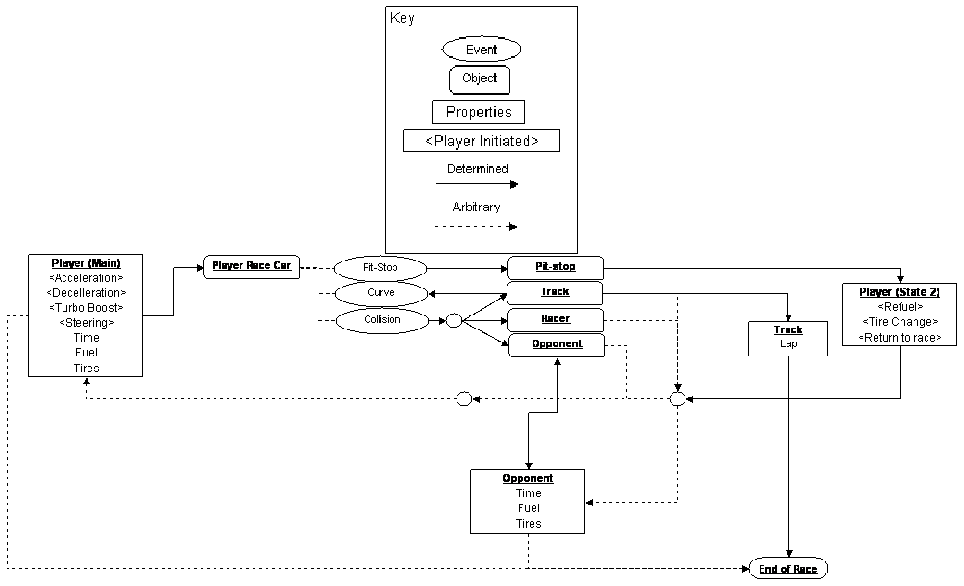
\includegraphics[width=\linewidth,height=0.82\textheight,keepaspectratio]{figures/appendix-c-flow-chart.pdf}
\end{guidance}
% Write your text below.

\subsection{Hold the Door -- Game Flow Chart}

The flow chart below illustrates the complete operational loop of \textbf{Hold the Door}, representing the states, decision nodes, and transitions between player actions, zombie lifecycle, tower interactions, and fence preservation.

\begin{figure}[htbp]
\centering
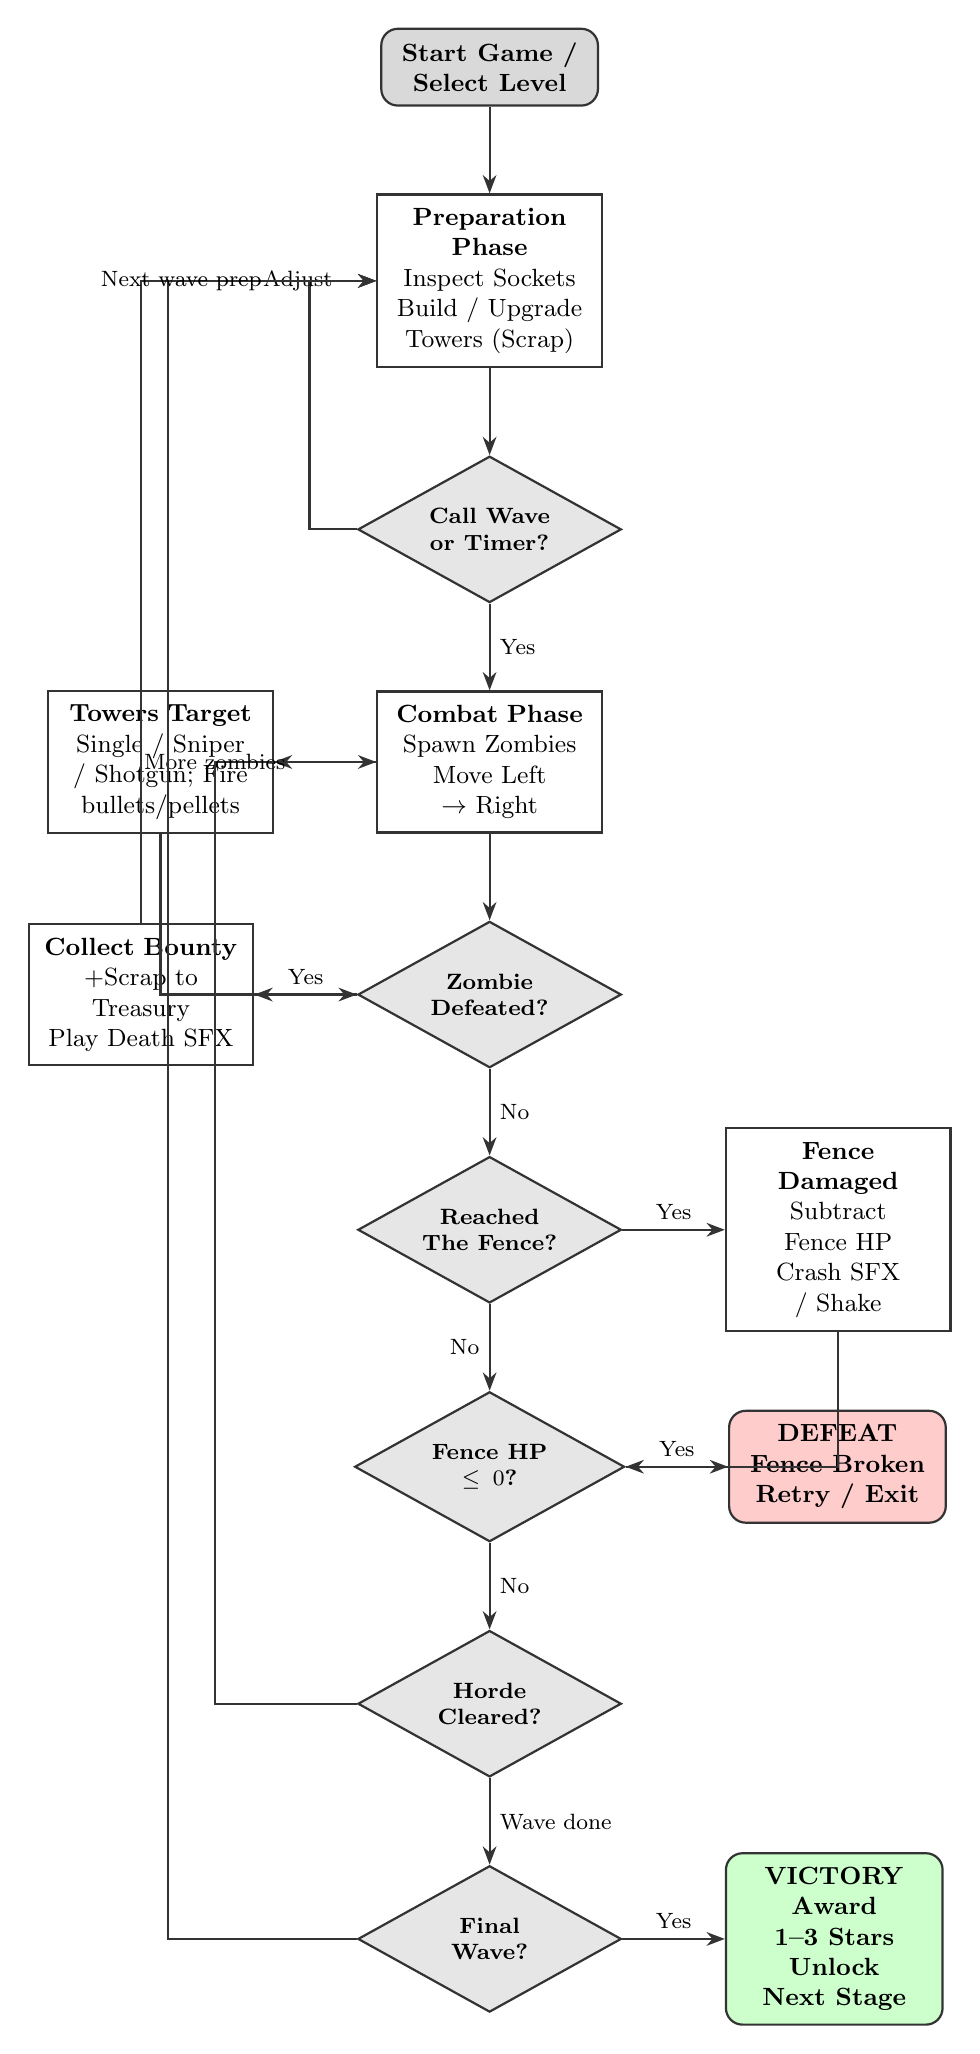
\begin{tikzpicture}[
  node distance=1.1cm and 1.3cm,
  terminal/.style={rectangle, rounded corners=6pt, draw=black!80, fill=gddhead, thick, text width=2.4cm, align=center, inner sep=5pt, font=\small\bfseries},
  process/.style={rectangle, draw=black!80, fill=white, thick, text width=2.5cm, align=center, inner sep=5pt, font=\small},
  decision/.style={diamond, aspect=1.8, draw=black!80, fill=gddlabel, thick, text width=2.0cm, align=center, inner sep=2pt, font=\footnotesize\bfseries},
  arrow/.style={-{Stealth[scale=1.0]}, thick, draw=black!80}
]

% Nodes
\node (start) [terminal] {Start Game / Select Level};
\node (prep) [process, below=of start] {\textbf{Preparation Phase}\\Inspect Sockets\\Build / Upgrade\\Towers (Scrap)};
\node (call) [decision, below=of prep] {Call Wave\\or Timer?};
\node (combat) [process, below=of call] {\textbf{Combat Phase}\\Spawn Zombies\\Move Left $\rightarrow$ Right};
\node (tower) [process, left=of combat] {\textbf{Towers Target}\\Single / Sniper / Shotgun; Fire bullets/pellets};
\node (hit) [decision, below=of combat] {Zombie\\Defeated?};
\node (bounty) [process, left=of hit] {\textbf{Collect Bounty}\\+Scrap to Treasury\\Play Death SFX};
\node (reach) [decision, below=of hit] {Reached\\The Fence?};
\node (dmg) [process, right=of reach] {\textbf{Fence Damaged}\\Subtract Fence HP\\Crash SFX / Shake};
\node (dead) [decision, below=of reach] {Fence HP\\$\le 0$?};
\node (defeat) [terminal, right=of dead, fill=red!20] {\textbf{DEFEAT}\\Fence Broken\\Retry / Exit};
\node (wavecheck) [decision, below=of dead] {Horde\\Cleared?};
\node (lastwave) [decision, below=of wavecheck] {Final\\Wave?};
\node (victory) [terminal, right=of lastwave, fill=green!20] {\textbf{VICTORY}\\Award 1--3 Stars\\Unlock Next Stage};

% Connections
\draw [arrow] (start) -- (prep);
\draw [arrow] (prep) -- (call);
\draw [arrow] (call) -- node[right, font=\footnotesize] {Yes} (combat);
\draw [arrow] (call.west) -- ++(-0.6,0) |- node[near end, left, font=\footnotesize] {Adjust} (prep.west);

\draw [arrow] (combat) -- (hit);
\draw [arrow] (combat.west) -- (tower.east);
\draw [arrow] (tower.south) |- (hit.west);

\draw [arrow] (hit) -- node[above, font=\footnotesize] {Yes} (bounty);
\draw [arrow] (bounty.north) |- (prep.west);
\draw [arrow] (hit) -- node[right, font=\footnotesize] {No} (reach);

\draw [arrow] (reach) -- node[above, font=\footnotesize] {Yes} (dmg);
\draw [arrow] (dmg) |- (dead);
\draw [arrow] (reach) -- node[left, font=\footnotesize] {No} (dead);

\draw [arrow] (dead) -- node[above, font=\footnotesize] {Yes} (defeat);
\draw [arrow] (dead) -- node[right, font=\footnotesize] {No} (wavecheck);

\draw [arrow] (wavecheck.west) -- ++(-1.8,0) |- node[near end, left, font=\footnotesize] {More zombies} (combat.west);
\draw [arrow] (wavecheck) -- node[right, font=\footnotesize] {Wave done} (lastwave);

\draw [arrow] (lastwave) -- node[above, font=\footnotesize] {Yes} (victory);
\draw [arrow] (lastwave.west) -- ++(-2.4,0) |- node[near end, left, font=\footnotesize] {Next wave prep} (prep.west);

\end{tikzpicture}
\caption{System Gameplay Flowchart of \textbf{Hold the Door}}
\label{fig:game-flowchart}
\end{figure}

% 8 Appendix D
\section{Appendix D}

\begin{guidance}
\centering
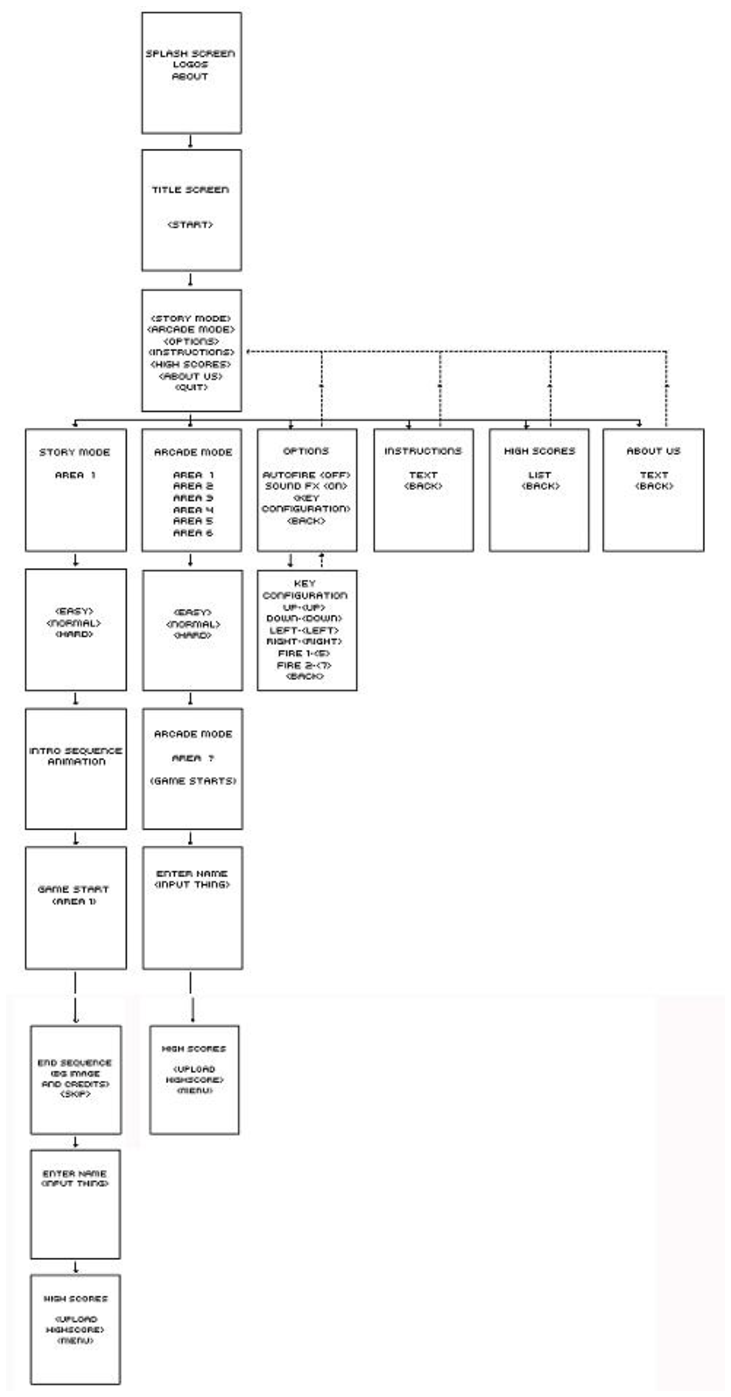
\includegraphics[width=\linewidth,height=0.82\textheight,keepaspectratio]{figures/appendix-d-game-architecture.pdf}
\end{guidance}
% Write your text below.

\subsection{Hold the Door -- Game Architecture Diagram}

The architecture diagram below outlines the screen hierarchy, UI navigation paths, and backend subsystem relationships governing the runtime lifecycle of \textbf{Hold the Door}.

\begin{figure}[htbp]
\centering
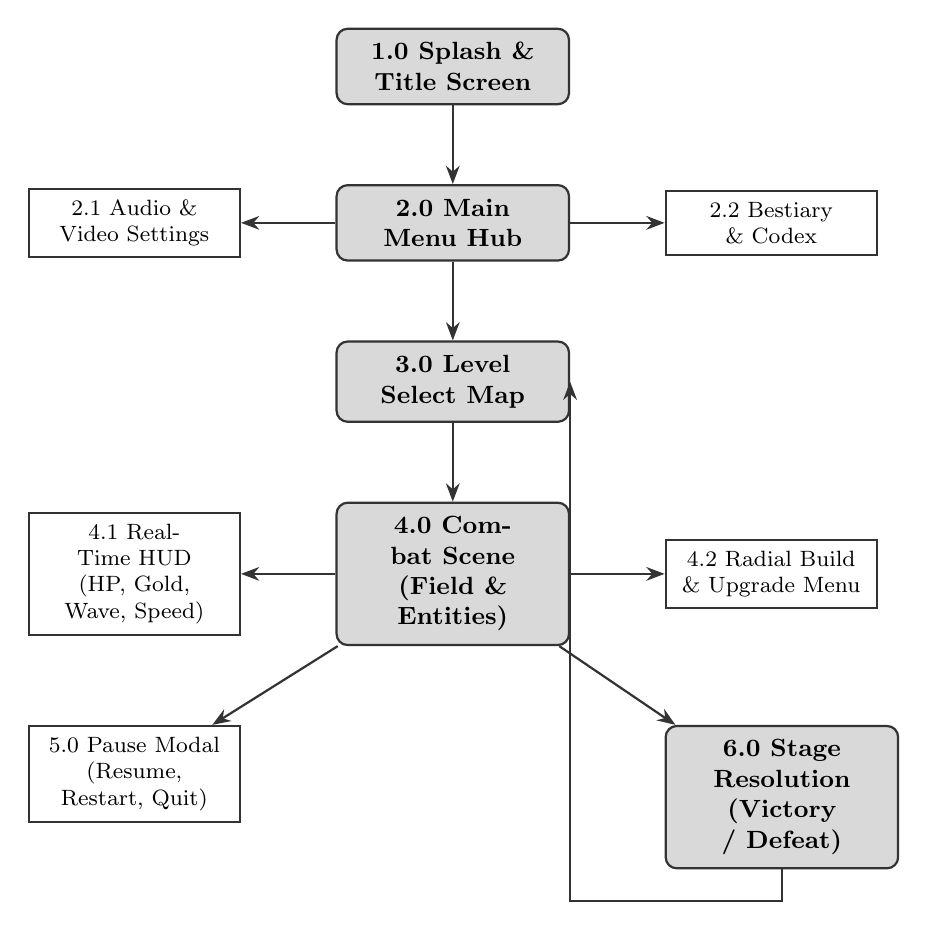
\begin{tikzpicture}[
  node distance=1.0cm and 1.2cm,
  screen/.style={rectangle, rounded corners=4pt, draw=black!80, fill=gddhead, thick, text width=2.6cm, align=center, inner sep=5pt, font=\small\bfseries},
  subscreen/.style={rectangle, draw=black!80, fill=white, thick, text width=2.4cm, align=center, inner sep=4pt, font=\footnotesize},
  system/.style={rectangle, rounded corners=2pt, draw=blue!70, fill=blue!5, thick, text width=2.5cm, align=center, inner sep=4pt, font=\footnotesize},
  arrow/.style={-{Stealth[scale=1.0]}, thick, draw=black!80}
]

% Screen Hierarchy
\node (title) [screen] {1.0 Splash \& Title Screen};
\node (menu) [screen, below=of title] {2.0 Main Menu Hub};
\node (settings) [subscreen, left=of menu] {2.1 Audio \& Video Settings};
\node (bestiary) [subscreen, right=of menu] {2.2 Bestiary \& Codex};
\node (levelselect) [screen, below=of menu] {3.0 Level Select Map};
\node (gameplay) [screen, below=of levelselect] {4.0 Combat Scene\\(Field \& Entities)};
\node (hud) [subscreen, left=of gameplay] {4.1 Real-Time HUD\\(HP, Gold, Wave, Speed)};
\node (radial) [subscreen, right=of gameplay] {4.2 Radial Build \& Upgrade Menu};
\node (pause) [subscreen, below left=of gameplay] {5.0 Pause Modal\\(Resume, Restart, Quit)};
\node (results) [screen, below right=of gameplay] {6.0 Stage Resolution\\(Victory / Defeat)};

% Screen Connections
\draw [arrow] (title) -- (menu);
\draw [arrow] (menu) -- (settings);
\draw [arrow] (menu) -- (bestiary);
\draw [arrow] (menu) -- (levelselect);
\draw [arrow] (levelselect) -- (gameplay);
\draw [arrow] (gameplay) -- (hud);
\draw [arrow] (gameplay) -- (radial);
\draw [arrow] (gameplay) -- (pause);
\draw [arrow] (gameplay) -- (results);
\draw [arrow] (results.south) -- ++(0,-0.4) -| (levelselect.east);

\end{tikzpicture}
\caption{Screen Hierarchy and UI Flow of \textbf{Hold the Door}}
\label{fig:screen-hierarchy}
\end{figure}

\subsection{Backend Software Subsystems}

The core Unity~6 execution layer is partitioned into decoupled singletons and ScriptableObjects communicating via C\# event delegates:

\begin{figure}[htbp]
\centering
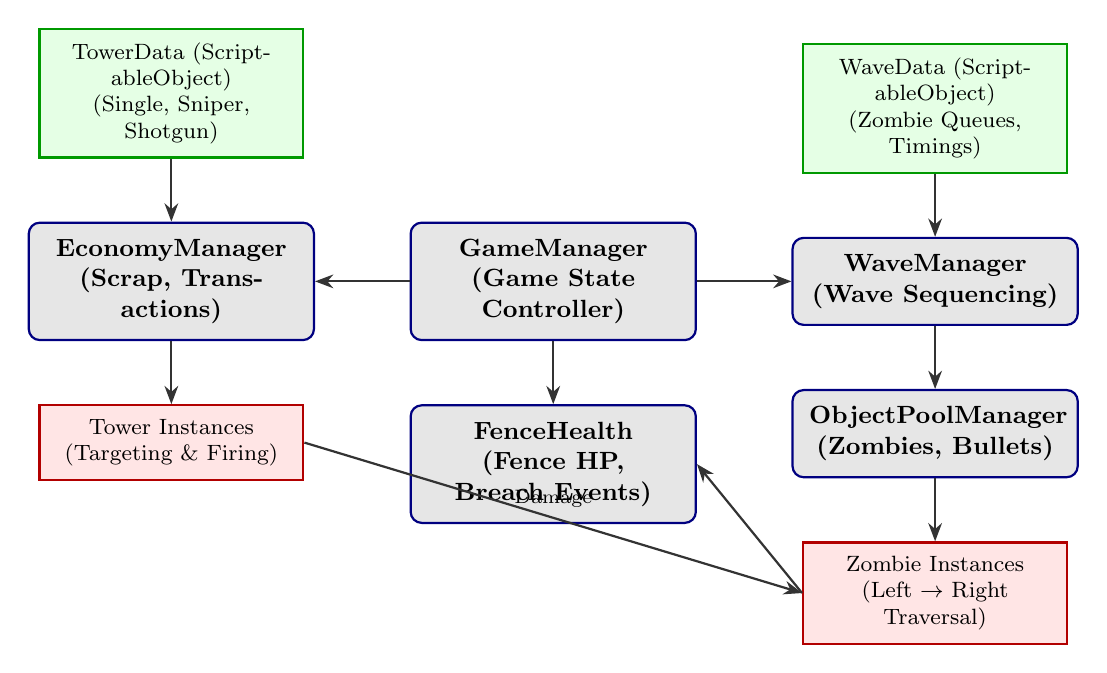
\begin{tikzpicture}[
  node distance=0.8cm and 1.2cm,
  mgr/.style={rectangle, rounded corners=4pt, draw=gddnavy, fill=gddlabel, thick, text width=3.2cm, align=center, inner sep=6pt, font=\small\bfseries},
  data/.style={rectangle, draw=green!60!black, fill=green!10, thick, text width=3.0cm, align=center, inner sep=5pt, font=\footnotesize},
  entity/.style={rectangle, draw=red!70!black, fill=red!10, thick, text width=3.0cm, align=center, inner sep=5pt, font=\footnotesize},
  arrow/.style={-{Stealth[scale=1.0]}, thick, draw=black!80}
]

\node (gm) [mgr] {GameManager\\(Game State Controller)};
\node (econ) [mgr, left=of gm] {EconomyManager\\(Scrap, Transactions)};
\node (wave) [mgr, right=of gm] {WaveManager\\(Wave Sequencing)};
\node (door) [mgr, below=of gm] {FenceHealth\\(Fence HP, Breach Events)};

\node (waveso) [data, above=of wave] {WaveData (ScriptableObject)\\(Zombie Queues, Timings)};
\node (towerso) [data, above=of econ] {TowerData (ScriptableObject)\\(Single, Sniper, Shotgun)};

\node (pool) [mgr, below=of wave] {ObjectPoolManager\\(Zombies, Bullets)};
\node (towers) [entity, below=of econ] {Tower Instances\\(Targeting \& Firing)};
\node (enemies) [entity, below=of pool] {Zombie Instances\\(Left $\rightarrow$ Right Traversal)};

\draw [arrow] (gm) -- (econ);
\draw [arrow] (gm) -- (wave);
\draw [arrow] (gm) -- (door);
\draw [arrow] (waveso) -- (wave);
\draw [arrow] (towerso) -- (econ);
\draw [arrow] (wave) -- (pool);
\draw [arrow] (pool) -- (enemies);
\draw [arrow] (econ) -- (towers);
\draw [arrow] (enemies.west) -- (door.east);
\draw [arrow] (towers.east) -- node[above, font=\scriptsize] {Damage} (enemies.west);

\end{tikzpicture}
\caption{Decoupled Software Subsystem and Event Architecture}
\label{fig:software-architecture}
\end{figure}

% 9 Appendix E: write your text below the grey guidance boxes (guidance environments).
\section{Appendix E}

\subsection{AI Use Declaration}

\begin{guidance}
Declare every AI tool used in the project in the table below. At the midterm the table covers the Concept Document and the Project Plan; in the final report it covers the whole project (code, assets, promotional materials and this document). The allowed levels and rules are given in the project announcements.

\begin{itemize}[label=\textbullet]
  \item Tool: the product name and, if you chose one, the mode or setting (e.g. ChatGPT – Auto, GitHub Copilot – Visual Studio, Unity AI Assistant). Give the model or version only if the tool shows it.
  \item The spell-check of your editor (e.g. Overleaf) needs no declaration.
  \item Export important chats as PDF or Markdown and submit them in the AI\_Logs folder; chat links are not accepted.
  \item AI-generated figures carry the tool name and “AI-generated” in their caption; commits with AI-generated code carry an “AI-assisted: \textless{}tool\textgreater{}” line in their message.
\end{itemize}
\end{guidance}
% Write your text below.

The table below declares the AI assistance utilized during the conceptualization, documentation structure design, and mathematical balancing of \textbf{Hold the Door}, compliant with Istanbul Sabahattin Zaim University YAM~415 academic guidelines.

\begin{longtblr}[theme=gdd, entry=none, label=none]{colspec={X[1.200,l]X[0.675,l]X[1.050,l]X[1.275,l]X[1.125,l]X[0.675,l]}, hlines, vlines, rowhead=1, row{1}={bg=gddhead}, cells={font=\small}}
\textbf{Tool and setting} & \textbf{Date} & \textbf{Purpose} & \textbf{Where used (section, file, asset)} & \textbf{How checked / changed} & \textbf{Member} \\
\fillrow[1.6em]Google Antigravity & 27.10.2026 & GCDD LaTeX formatting and structuring & All sections (\texttt{main.tex}, Sections 2--4, App B--D) & Verified against YAM415 template requirements & Emir KAYA \\
\fillrow[1.6em]Google Antigravity & 27.10.2026 & Mathematical curve and balance pass & Section 3, Section 4, Appendix B & Adjusted damage and gold pacing manually & Ömer Faruk YÜCE \\
\fillrow[1.6em]Google Antigravity & 27.10.2026 & TikZ flowchart \& architecture mapping & Appendix C, Appendix D & Reviewed visual transitions and state accuracy & Metehan GERGİN \\
\end{longtblr}

\noindent\checkbox~No AI tool was used in the project or in this document.

\end{document}
